\section{Polymers and Micelles}
\label{sect:Polymers_Micelles}

\subsection{Gaussian chain}
\label{sect:GaussCoil}
~\\

\begin{figure}[htb]
\begin{center}
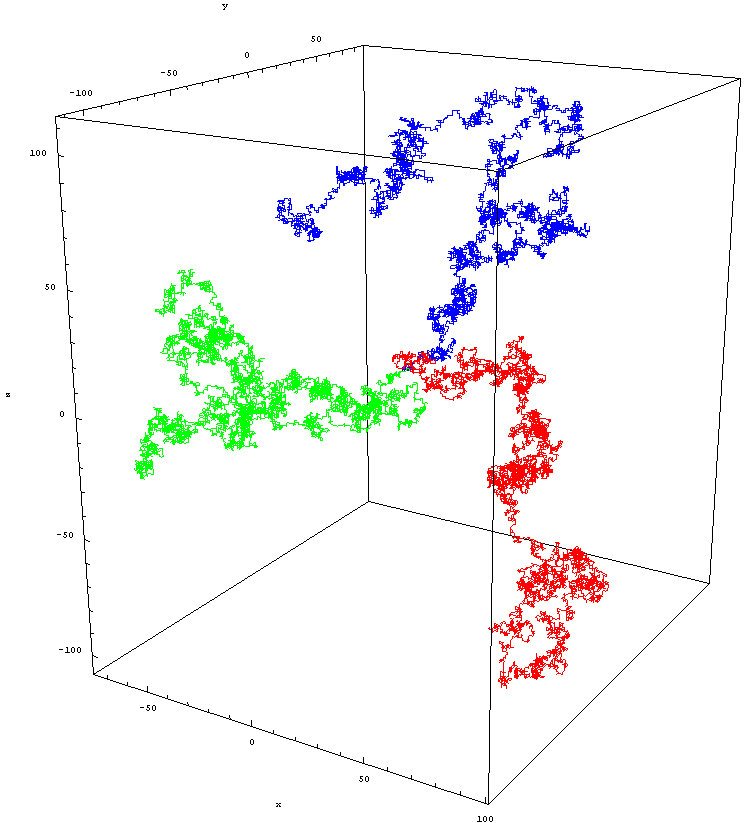
\includegraphics[width=0.744\textwidth]{Walk3d_0.png}
\end{center}
\caption{The underlying model for a polymer chain is an
isotropic random walk on the Euclidean lattice $\mathbb{Z}^3$.
This picture shows three different walks after 10 000 unit steps,
all three starting from the origin. \label{fig:RandomWalk3D}}
\end{figure}

Consider a flexible polymer coil where each monomer located at a
distance $\mathbf{R}_m$ its scattering field amplitude is given by
\begin{align}
F(\mathbf{q},t) &= \sum_{m=1}^N e^{-\imath
\mathbf{q}\cdot\mathbf{R}_m(t)} .
\end{align}
The scattering intensity averaged over all molecule configurations
reads
\begin{align}
\left\langle \abs{F(\mathbf{q})}^2\right\rangle
&= \sum_{m,n} \left\langle e^{-\imath\mathbf{q}\cdot(\mathbf{R}_m-\mathbf{R}_n)} \right\rangle
\end{align}
As the monomer segments $\mathbf{R}_m-\mathbf{R}_n$ are Gaussian distributed
the averages $\langle\cdots\rangle$ can be written as
\begin{subequations}
\begin{align}
\left\langle e^{-\imath\mathbf{q}\cdot(\mathbf{R}_m-\mathbf{R}_n)} \right\rangle
&= e^{\frac{q^2}{6}\left\langle \left( \mathbf{R}_m-\mathbf{R}_n\right)^2\right\rangle} \\
&= e^{-\frac{q^2b^2}{6}\abs{m-n}^{2\nu}}
\end{align}
\end{subequations}
Here $b$ is the statistical segment length and the contour length $L$ equals $L=Nb$.
The average of the segment inter-distances squares is kept in the general form
\begin{align}
\left\langle \left( \mathbf{R}_m-\mathbf{R}_n\right)^2\right\rangle
&= b^2 \abs{m-n}^{2\nu}.
\end{align}
$\nu$ is the excluded volume parameter from the Flory mean field
theory\footnote{P.J. Flory, "Statistical Mechanics of Chain Molecules", Interscience Publishers (1969)}\footnote{\href{http://www.ncnr.nist.gov/staff/hammouda/the_SANS_toolbox.pdf}{Boualem Hammouda, \texttt{the\_SANS\_toolbox.pdf}}}
of polymer solutions. The radius of gyration $R_G$ is given by
\begin{subequations}
\begin{align}
R_G^2 &= \frac{1}{2N^2}\sum_{m,n}^N \left\langle \left( \mathbf{R}_m-\mathbf{R}_n\right)^2\right\rangle \\
      &= \frac{1}{2N^2}\sum_{m,n}^N b^2 \abs{m-n}^{2\nu} \\
      &= \frac{b^2}{N} \sum_k^N \left(1-\frac{k}{N}\right) k^{2\nu} \\
      &= \frac{b^2}{\left(2\nu+1\right)\left(2\nu+2\right)} N^{2\nu}
\end{align}
\end{subequations}
Three cases are relevant:
\begin{enumerate}
\item Self-avoiding walk corresponds to swollen chains with $\nu = 3/5$, for which
$R_G^2=\frac{25}{176}b^2N^{6/5}$.
\item Pure random walk corresponds to chains in $\Theta$-conditions (where solvent-solvent,
monomer-monomer and solvent-monomer interactions are equivalent) with $\nu = 1/2$,
for which $R_G^2=\frac{1}{6}b^2N$.
\item Self attracting walk corresponds to collapsed chains with $\nu = 1/3$, for which
$R_G^2=\frac{9}{40}b^2N^{2/3}$.
\end{enumerate}
Using the general identity
\begin{align}
\sum_{i,j}^N y(\abs{i-j}) = N+2\sum_{k=1}^N(N-k) y(k)
\end{align}
the form factor reads
\begin{align}
P(q) &= \frac{1}{N^2}\abs{F(q)}^2 = \frac{1}{N^2}
\left\{N+2\sum_{k=1}^N(N-k)e^{-\frac{q^2b^2}{6}k^{2\nu}} \right\}
\end{align}
Going to the continuous limit $(N \gg 1)$, one obtains:
\begin{subequations}
\begin{align}
P(q) &= 2\int_0^1 \mathrm{d}x \; (1-x)e^{-\frac{q^2b^2}{6}N^{2\nu}x^{2\nu}} \\
&= \frac{U^{\frac{1}{2 \nu}} \Gamma\left(\frac{1}{2 \nu}\right)-
\Gamma\left(\frac{1}{\nu}\right)-U^{\frac{1}{2\nu}}
\Gamma\left(\frac{1}{2 \nu},U\right)+\Gamma\left(\frac{1}{\nu},U\right)}{\nu U^{1/\nu}} \\
&= \frac{1}{\nu U^{\frac{1}{2 \nu}}} \; \gamma\left(\frac{1}{2 \nu},U\right)-
   \frac{1}{\nu U^{\frac{1}{\nu}}}   \; \gamma\left(\frac{1}{  \nu},U\right)
\label{eq:generalizedGauss}
\end{align}
\end{subequations}
with the modified variable
\begin{align}
U&=\frac{q^2b^2N^{2\nu}}{6} = \left(2\nu+1\right)\left(2\nu+2\right)\frac{q^2R_G^2}{6}
\label{eq:Uexclvol}
\end{align}
and the upper incomplete Gamma Function $\Gamma(a,x) = \int_x^\infty \mathrm{d}t \; t^{a-1} \exp(-t)$ and lower incomplete Gamma Function $\gamma(a,x) = \int_0^x \mathrm{d}t \; t^{a-1} \exp(-t)$
for $a$ real and $x \geq 0$ and the Gamma function $\Gamma(a)=\Gamma(a,0)=\gamma(a,\infty)= \Gamma(a,x)+\gamma(a,x)=\int_0^\infty \mathrm{d}t\;  t^{a-1} \exp(-t)$.
Polymer chains follow Gaussian statistics in polymer solutions: they are swollen in good
solvents $\nu=3/5$, are thermally relaxed in "theta"-solvents $\nu=1/2$ and partially precipitate in poor solvents $\nu=1/3$.
The familiar Debye function is recovered when $\nu = 1/2$. The asymptotic limit at large $q$-values of the generalized
Gaussian chain is dominated by the $\frac{1}{\nu U^{\frac{1}{2\nu}}}\Gamma\left(\frac{1}{2\nu}\right)$
term which varies like $U^{-1/(2\nu)} \sim q^{-1/\nu}$. For $\nu =1$ we get the limit of an infinitesimal thin rod
and for $\nu=1/4$ a compact object with a Porod law of $q^{-4}$.

\SASfit has implemented the generalized form of a Gaussian (\texttt{generalized Gaussian coil}) coil and the standard
Debye formula \texttt{Gauss}. In both cases three versions are implemented which only differ in their parametrization of the forward scattering. In case of the Debye-formula also the polydisperse \texttt{GaussPoly} is implemented.

\textcolor[rgb]{1.00,1.00,1.00}{Gauss}\\
\subsubsection{Gauss }
\label{sect:Gauss}
~\\
Flexible polymer chains which are not self-avoiding
and obey Gaussian statistics. Debye (1947) \cite{Debye1947} has calculated the form factor of such
chains:
\begin{align}
I_\text{Gauss}(q) &= I_0 2\frac{\exp(-u)+u-1}{u^2} \label{eq:DebyeGauss}\\
u &= q^2R_g^2
\end{align}

\vspace{5mm}
\uline{Input Parameters for model \texttt{Gauss}:}
\begin{description}
\item[\texttt{Rg}] radius of gyration $R_g$
\item[\texttt{I0}] forward scattering $I_0$ for $q=0$
\end{description}
\vspace{5mm}

\textcolor[rgb]{1.00,1.00,1.00}{Gauss}\\
\subsubsection{Gauss2}
\label{sect:Gauss2}
~\\
This form factor \cite{Debye1947} differs only by the parametrization for the forward scattering
$I_0=(b_p-V\eta_\text{s})^2$ from the Debye formula in eq.\ \ref{eq:DebyeGauss}
\begin{align}
I_\text{Gauss2}(q) &= \beta^2 2\frac{\exp(-u)+u-1}{u^2} \\
u &= q^2R_g^2 \nonumber \\
\beta &= b_p-V\eta_\text{s}, \nonumber
\end{align}
where $b_p$ is the scattering length of a polymer molecule of molecular volume $V$ dissolved in a solvent
of scattering length density $\eta_\text{s}$ from which the excess scattering length of a polymer molecule
$\beta$ can be calculated. Combining this form factor with a \texttt{Delta} size distribution \ref{sec:Delta}
is needed to scale the scattering intensity. With proper values for the form factor the parameter $N$
of the \texttt{Delta}-distribution yields the particle number density.

\vspace{5mm}
\uline{Input Parameters for model \texttt{Gauss2}:}
\begin{description}
\item[\texttt{Rg}] radius of gyration $R_g$
\item[\texttt{b\_p}] scattering length of polymer $b_p$ in [cm]
\item[\texttt{V}] molecular volume of a single polymer molecule $V$ in [cm$^3$]
\item[\texttt{eta\_s}] scattering length density of solvent $\eta_\text{s}$ in [cm$^{-2}$]
\end{description}

\textcolor[rgb]{1.00,1.00,1.00}{Gauss}\\
\subsubsection{Gauss3}
\label{sect:Gauss3}
~\\
This form factor  \cite{Debye1947} differs only by the parametrization for the forward scattering
$I_0=(b_p-\frac{M_w}{N_a\rho_p}\eta_\text{s})^2$ from the Debye formula in eq.\ \ref{eq:DebyeGauss}
\begin{align}
I_\text{Gauss3}(q) &= \beta^2 2\frac{\exp(-u)+u-1}{u^2}
\end{align}
with
\begin{align}
u &= q^2R_g^2 \nonumber \\
\beta &= b_p-V\eta_\text{s} \nonumber\\
V &= \frac{M_w}{N_a\rho_p} \nonumber \\
N_a &= \mbox{Avogadro number} \nonumber
\end{align}

\uline{Input Parameters for model \texttt{Gauss3}:}
\begin{description}
\item[\texttt{Rg}] radius of gyration $R_g$
\item[\texttt{b\_p}] scattering length of polymer $b_p$ in [cm]
\item[\texttt{M\_w}] molecular weight of polymer $M_w$ in [g/mol]
\item[\texttt{rho\_p}] mass density of polymer $\rho_p$ in [g cm$^{-3}$]
\item[\texttt{eta\_s}] scattering length density of solvent $\eta_\text{s}$ in [cm$^{-2}$]
\end{description}

\begin{figure}[htb]
\begin{center}
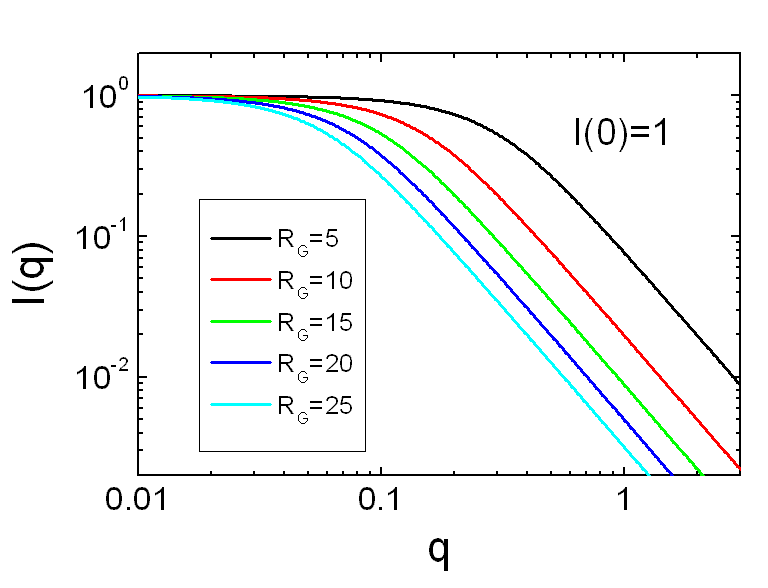
\includegraphics[width=0.768\textwidth]{gaussian_coils.png}
\end{center}
\caption{Scattering function of Gaussian coils plotted for several radii of gyration.}
\label{fig:I_gaussian_coils}
\end{figure}

\textcolor[rgb]{1.00,1.00,1.00}{Gauss}\\
\subsubsection{Polydisperse flexible polymers with Gaussian statistics} \cite{Pedersen2002}  \label{sect:GaussPoly}
~\\
Polydispersity has been included in terms of a Schulz–Zimm mass distribution by
Zimm (1948) \cite{zimm:1093}  and Greschner (1973) \cite{Greschner1973}
~\\

\begin{align}
I_\text{GaussPoly}(q) &= I_0 2 \frac{\left( 1+U x\right)^{-1/U}+x-1}{(1+U)x^2} \\
x &= q^2R_g^2/(1+2U) \nonumber \\
U &= \frac{M_w}{M_n} -1 \nonumber
\end{align}

\vspace{5mm}
\uline{Input Parameters for model \texttt{GaussPoly}:}
\begin{description}
\item[\texttt{Rg}] radius of gyration $R_g$
\item[\texttt{M\_w}] weight averaged molecular weight $M_w$
\item[\texttt{M\_n}] number averaged molecular weight $M_n$
\item[\texttt{I0}] forward scattering $I_0$ for $q=0$
\end{description}

\begin{figure}[htb]
\begin{center}
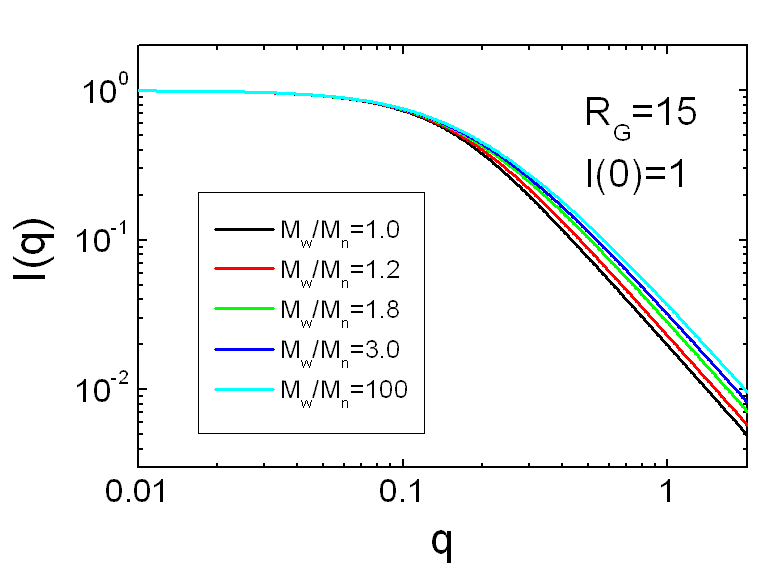
\includegraphics[width=0.768\textwidth]{gauss_poly.png}
\end{center}
\caption{Scattering function of polydisperse Gaussian coil plotted for several ratios of $M_w/M_n$.}
\label{fig:I_gauss_poly}
\end{figure}

\textcolor[rgb]{1.00,1.00,1.00}{Gauss}\\
\subsubsection{generalized Gaussian coil} \cite{Hammouda,Hammouda2012,Hammouda1993,Hammouda2016}
\label{sect:generalized_gaussian_coil}
~\\
The scattering function for the generalized Gaussian coil is according to eq.\ \ref{eq:generalizedGauss}
\begin{align}
I_\text{gGc}(q) &= I_0
\left(
\frac{1}{\nu U^{\frac{1}{2 \nu}}} \; \gamma\left(\frac{1}{2 \nu},U\right)-
\frac{1}{\nu U^{\frac{1}{  \nu}}} \; \gamma\left(\frac{1}{  \nu},U\right)
\right)
\label{eq:generalizedGauss1}
\end{align}
with the modified variable
\begin{align}
U&= \left(2\nu+1\right)\left(2\nu+2\right)\frac{q^2R_G^2}{6}
\end{align}
and the lower incomplete Gamma Function $\gamma(a,x) = \int_0^x \mathrm{d}t \; t^{a-1} \exp(-t)$.
$\nu$ is the excluded volume parameter from the Flory mean field theory and typical values for them are
\begin{description}
\item[$\nu=1/3$] partially precipitate in poor solvents
\item[$\nu=1/2$] thermally relaxed in "theta"-solvents
\item[$\nu=3/5$] swollen in good solvents
\end{description}

\vspace{5mm}
\noindent \uline{Input Parameters for model \texttt{generalized Gaussian coil}:}
\begin{description}
\item[\texttt{Rg}] radius of gyration $R_g$
\item[\texttt{nu}] excluded volume parameter $\nu>0$
\item[\texttt{I0}] forward scattering $I_0$ for $q=0$
\end{description}
\vspace{5mm}

\noindent \uline{Note:}
\begin{itemize}
\item For large $q$-values to model decays with the law $\propto q^{-1/\nu}$ for $q \rightarrow 0$
\end{itemize}
\vspace{5mm}

\subsubsection{generalized Gaussian coil 2} \cite{Hammouda,Hammouda2012}
\label{sect:generalized_gaussian_coil2}
~\\
The scattering function for the generalized Gaussian coil is according to eq.\ \ref{eq:generalizedGauss}
and differs only by the parametrization for the forward scattering
$I_0=(b_p-V\eta_\text{s})^2$ from the formula in eq.\ \ref{eq:generalizedGauss1}
\begin{align}
I_\text{gGc2}(q) &= \left(b_p-V\eta_\text{s}\right)^2
\left(
\frac{1}{\nu U^{\frac{1}{2 \nu}}} \; \gamma\left(\frac{1}{2 \nu},U\right)-
\frac{1}{\nu U^{\frac{1}{  \nu}}} \; \gamma\left(\frac{1}{  \nu},U\right)
\right)
\label{eq:generalizedGauss2}
\end{align}
with the modified variable
\begin{align}
U&= \left(2\nu+1\right)\left(2\nu+2\right)\frac{q^2R_G^2}{6}
\end{align}

\vspace{5mm}
\noindent \uline{Input Parameters for model \texttt{generalized Gaussian coil 2}:}
\begin{description}
\item[\texttt{Rg}] radius of gyration $R_g$
\item[\texttt{b\_p}] scattering length of polymer $b_p$ in [cm]
\item[\texttt{V}] molecular volume of a single polymer molecule $V$ in [cm$^3$]
\item[\texttt{eta\_s}] scattering length density of solvent $\eta_\text{s}$ in [cm$^{-2}$]
\end{description}
\vspace{5mm}

\noindent \uline{Note:}
\begin{itemize}
\item For large $q$-values to model decays with the law $\propto q^{-1/\nu}$ for $q \rightarrow 0$
\end{itemize}
\vspace{5mm}

\subsubsection{generalized Gaussian coil 3} \cite{Hammouda,Hammouda2012}
\label{sect:generalized_gaussian_coil3}
~\\
The scattering function for the generalized Gaussian coil is according to eq.\ \ref{eq:generalizedGauss}
and differs only by the parametrization for the forward scattering
$I_0=(b_p-\frac{M_w}{N_a\rho_p}\eta_\text{s})^2$ from the formula in eq.\ \ref{eq:generalizedGauss1}
\begin{align}
I_\text{gGc3}(q) &= \left(b_p-\frac{M_w}{N_a\rho_p}\eta_\text{s}\right)^2
\left(
\frac{1}{\nu U^{\frac{1}{2 \nu}}} \; \gamma\left(\frac{1}{2 \nu},U\right)-
\frac{1}{\nu U^{\frac{1}{  \nu}}} \; \gamma\left(\frac{1}{  \nu},U\right)
\right)
\label{eq:generalizedGauss3}
\end{align}
with the modified variable
\begin{align}
U&= \left(2\nu+1\right)\left(2\nu+2\right)\frac{q^2R_G^2}{6}
\end{align}

\vspace{5mm}
\noindent \uline{Input Parameters for model \texttt{generalized Gaussian coil 3}:}
\begin{description}
\item[\texttt{Rg}] radius of gyration $R_g$
\item[\texttt{b\_p}] scattering length of polymer $b_p$ in [cm]
\item[\texttt{M\_w}] molecular weight of polymer $M_w$ in [g/mol]
\item[\texttt{rho\_p}] mass density of polymer $\rho_p$ in [g cm$^{-3}$]
\item[\texttt{eta\_s}] scattering length density of solvent $\eta_\text{s}$ in [cm$^{-2}$]
\end{description}
\vspace{5mm}

\noindent \uline{Note:}
\begin{itemize}
\item For large $q$-values to model decays with the law $\propto q^{-1/\nu}$ for $q \rightarrow 0$
\end{itemize}
\vspace{5mm}

\begin{figure}[htb]
\begin{center}
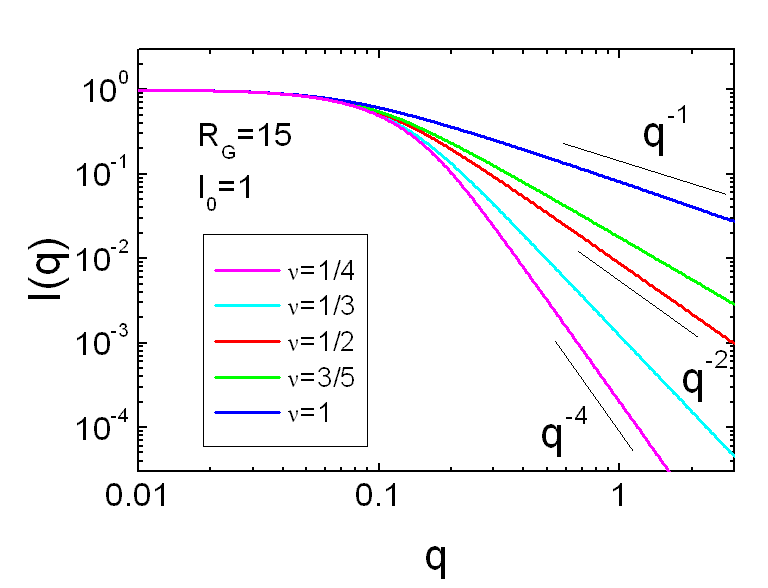
\includegraphics[width=0.768\textwidth,height=0.588\textwidth]{generalized_gaussian_coils.png}
\end{center}
\caption{Scattering function of the generalized Gaussian coil plotted for several excluded volume parameters.}
\label{fig:I_generalized_gaussian_coils}
\end{figure}

\clearpage
\subsection{Star-shaped polymers}
\label{sect:StarShapedPolymers}
~\\
Star-shaped polymers \cite{Wikipedia2018StarShapedPolymers} are branched polymers consisting of several (more than three) linear chains connected to a central core \cite{Ren2016}. The core of the star-shaped polymer is much smaller than the length of the arms and can be an atom, molecule, or macromolecule. Star-shaped polymers in which the arms are all equivalent in length and structure are considered homogeneous, and ones with variable lengths and structures are considered heterogeneous. For selected types of star-shaped polymers analytical expressions for the scattering intensity have been published and included in \SASfit.

~\\
\subsubsection{Star polymer with Gaussian statistic according to Benoit}
\label{sect:Benoit}
~\\

\begin{figure}[htb]
\begin{center}
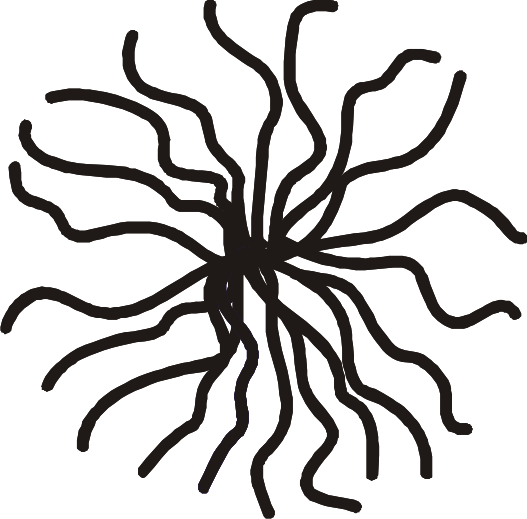
\includegraphics[width=0.2635\textwidth,height=0.2595\textwidth]{Benoit.png}
\end{center}
\caption{Sketch of a branched or star
polymers with $f$ number of arms} \label{fig:BenoitStar}
\end{figure}

Benoit \cite{Benoit53} derived an expression for the scattering from branched or star
polymers with a number of arms $f$, which can be expressed in the following way:
\begin{align}
I_\text{Star}(Q,R_G,f)= I_0 \frac{2}{f\nu^2}
    \left( \nu-\left[1-e^{-\nu}\right]+\frac{f-1}{2}\left[1-e^{-\nu}\right]^2\right)
\end{align}
with $\DS u=R_G^2Q^2$, $\DS \nu=\frac{uf}{3f-2}$ and $\DS
\lim_{Q=0}I_\text{Star}(Q,R_G,f)=I_0$. $f$
denotes the number of arms and $R_G$ the Guinier radius of a
single arm.

\vspace{5mm}

\noindent
\uline{Input Parameters for model \texttt{BenoitStar}:}
\begin{description}
\item[\texttt{I0}] forward scattering $I_0$ for $q=0$
\item[\texttt{RG}] radius of gyration of the star polymer $R_g$
\item[\texttt{dummy}] not used
\item[\texttt{dummy}] not used
\item[\texttt{f}] number of arms $f$
\end{description}


\begin{figure}[htb]
\begin{center}
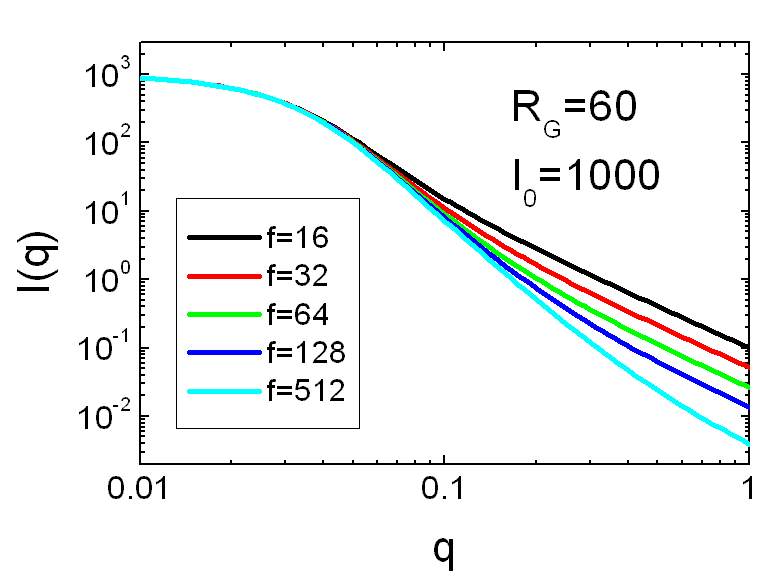
\includegraphics[width=0.768\textwidth,height=0.588\textwidth]{Benoit_Iq.png}
\end{center}
\caption{Scattering function of a star polymer according to Benoit. } \label{fig:Benoit_Iq}
\end{figure}

\clearpage

%\noindent REFERENCE:\\
%H.Benoit, J.Polym.Sci. 11(1953)507 \\

%%%%%%%%%%%%%%%%%%%%%%%%%%%%%%%%%%%%%%%%%%%%%%%%%%%%%%%%%%%%%%%%%%%%%
\clearpage
\subsubsection{Star polymer with arms of rigid rods}
\label{sect:StarRigidRods}
~\\
\cite{Huber1989}

\begin{figure}[htb]
\begin{center}
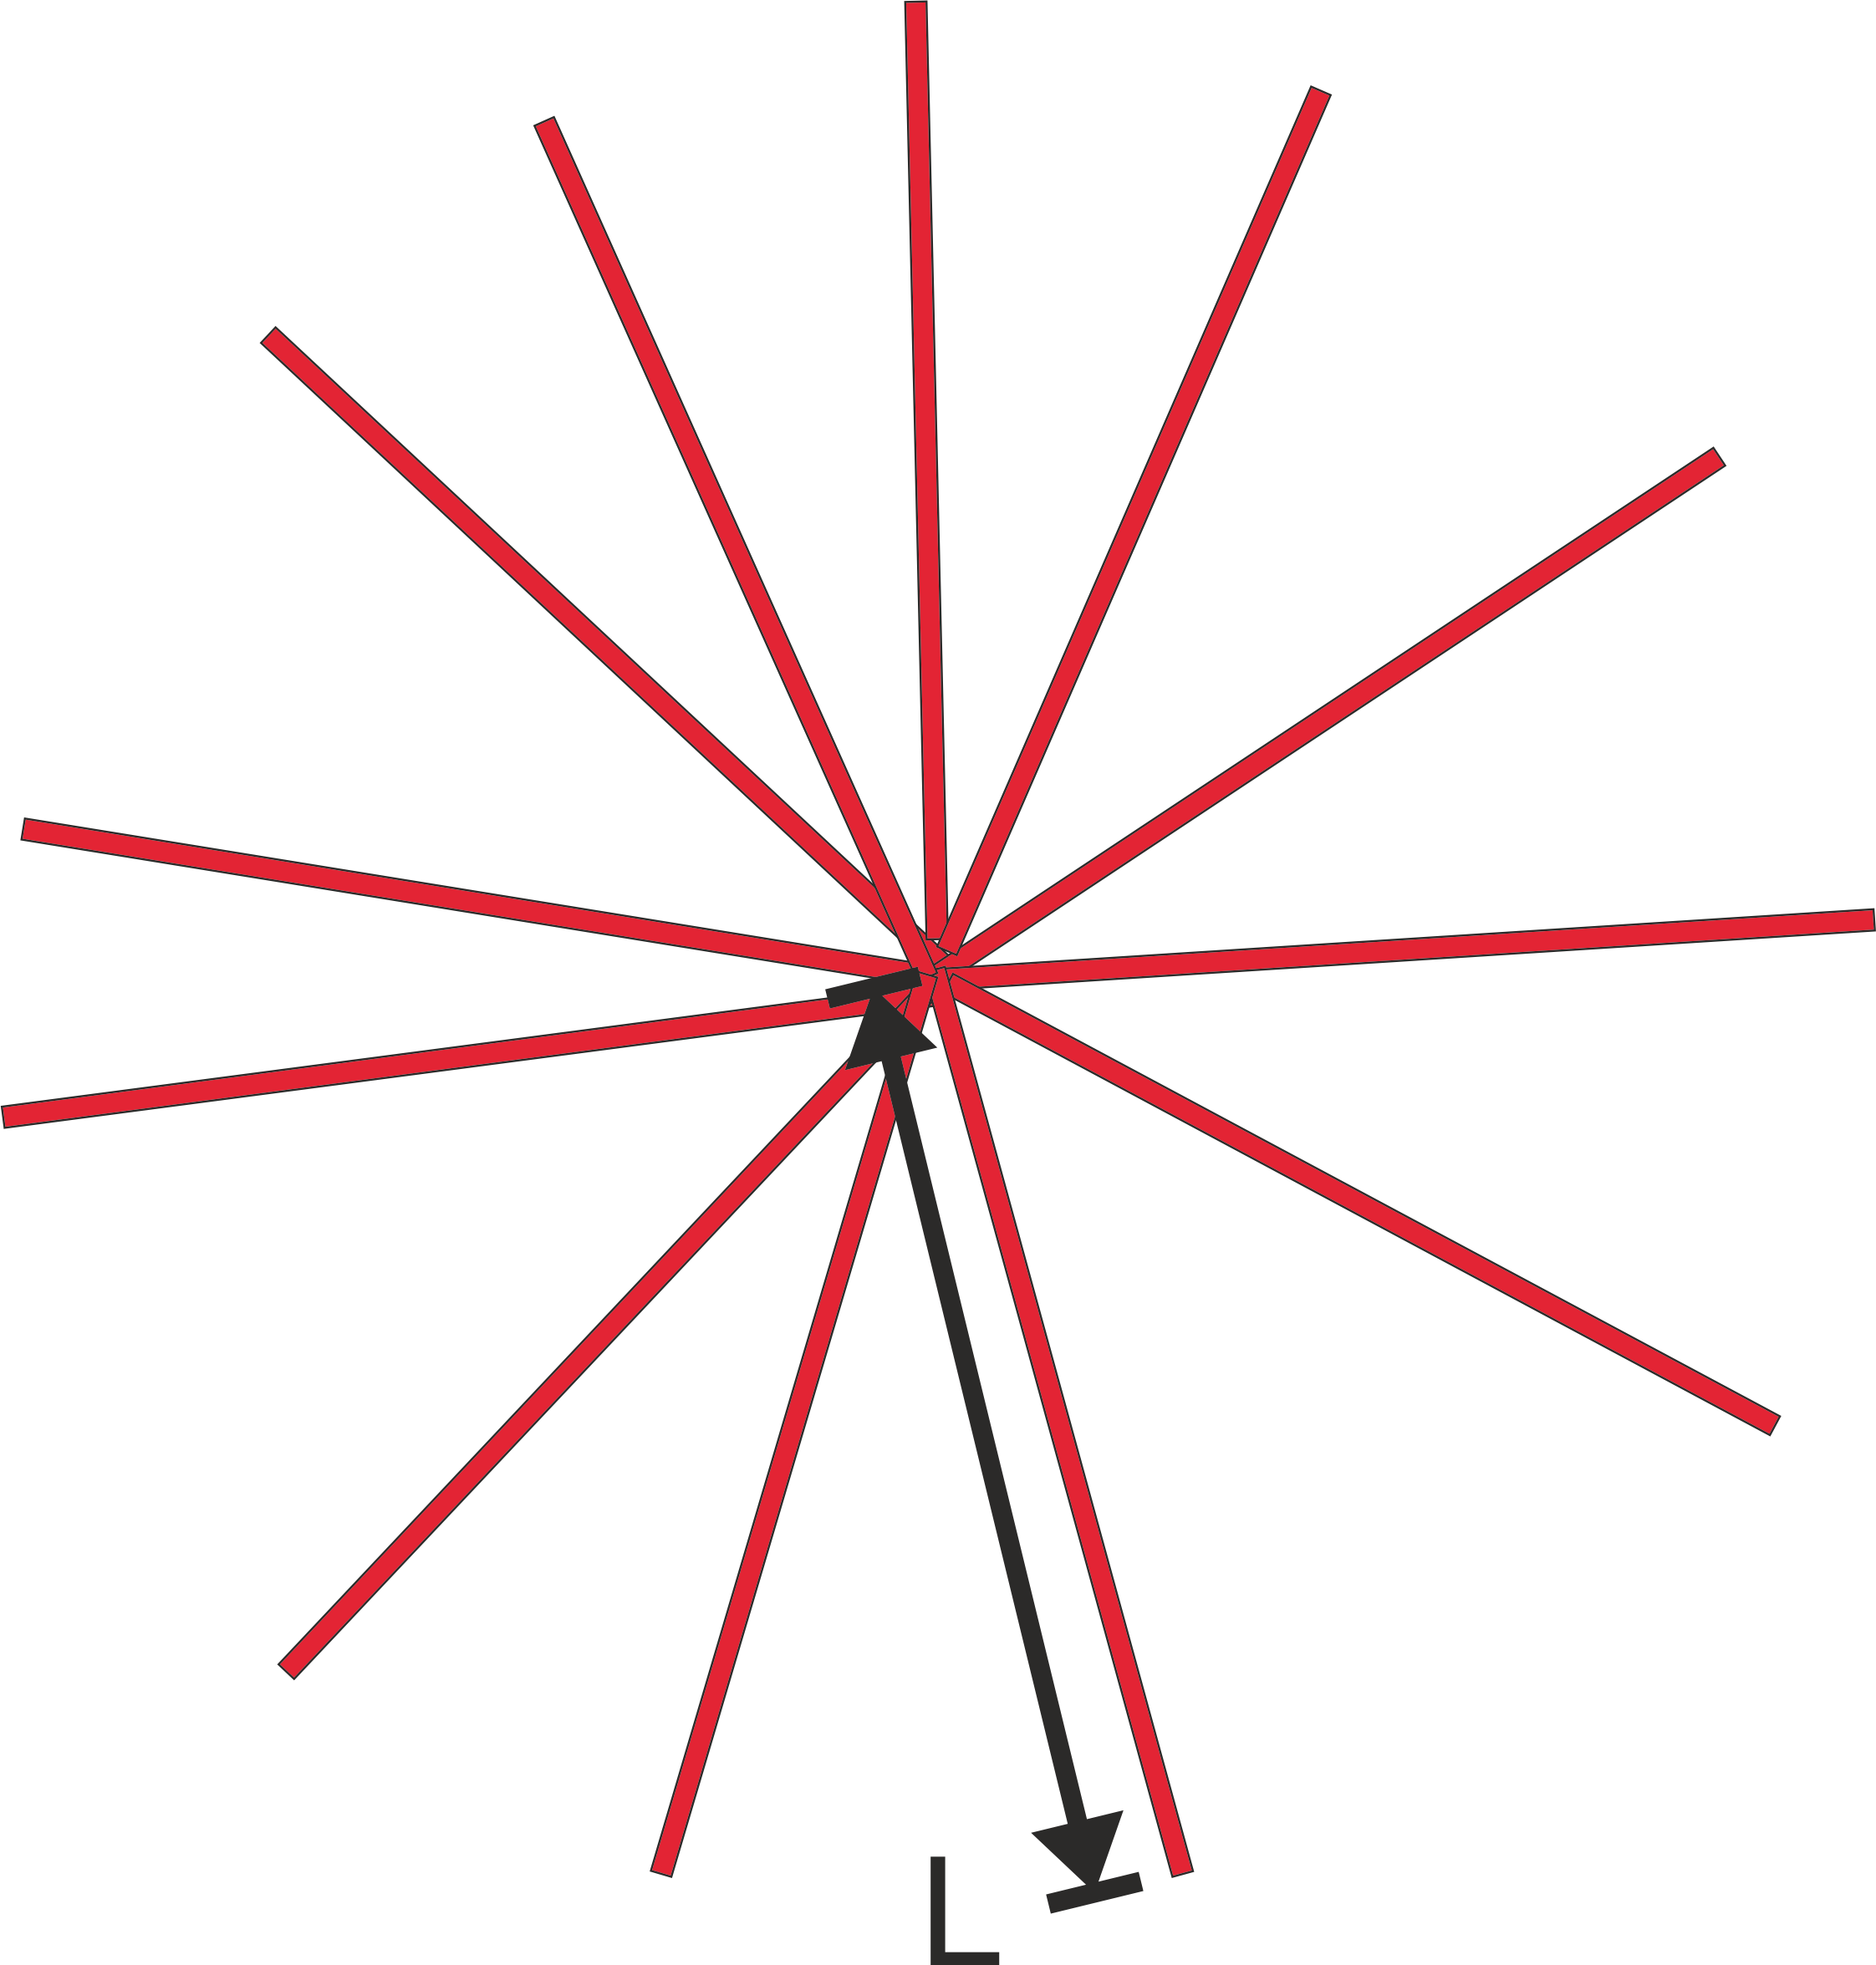
\includegraphics[width=0.5\textwidth]{broken_rods_star.png}
\end{center}
\caption{Star with arms of thin rigid rods} \label{fig:broken_rods_star}
\end{figure}

\begin{align}
 P_\mathrm{star}(Q) &= I_0/f\left(P_\mathrm{sb} + (f-1)P_\mathrm{ib} \right) \\
 P_\mathrm{sb} &= 2 \mathrm{Si}(qL)/(qL)-\mathrm{j}_0(qL/2) \\
 P_\mathrm{ib} &= \left( \mathrm{Si}(qL)/(qL)\right)^2
\end{align}
with $\mathrm{j}_0(x)=\frac{\sin(x)}{x}$ being the spherical Bessel function of first kind and zero order.

\vspace{5mm}

\noindent
\uline{Input Parameters for model \texttt{star polymer with arms of rigid rods}:}
\begin{description}
\item[\texttt{I0}] forward scattering $I_0$ for $q=0$
\item[\texttt{L}]length $L$ of a single rigid infinitesimal thin rodlike arm
\item[\texttt{dummy}] not used
\item[\texttt{dummy}] not used
\item[\texttt{f}] number of arms $f$
\end{description}

\begin{figure}[htb]
\begin{center}
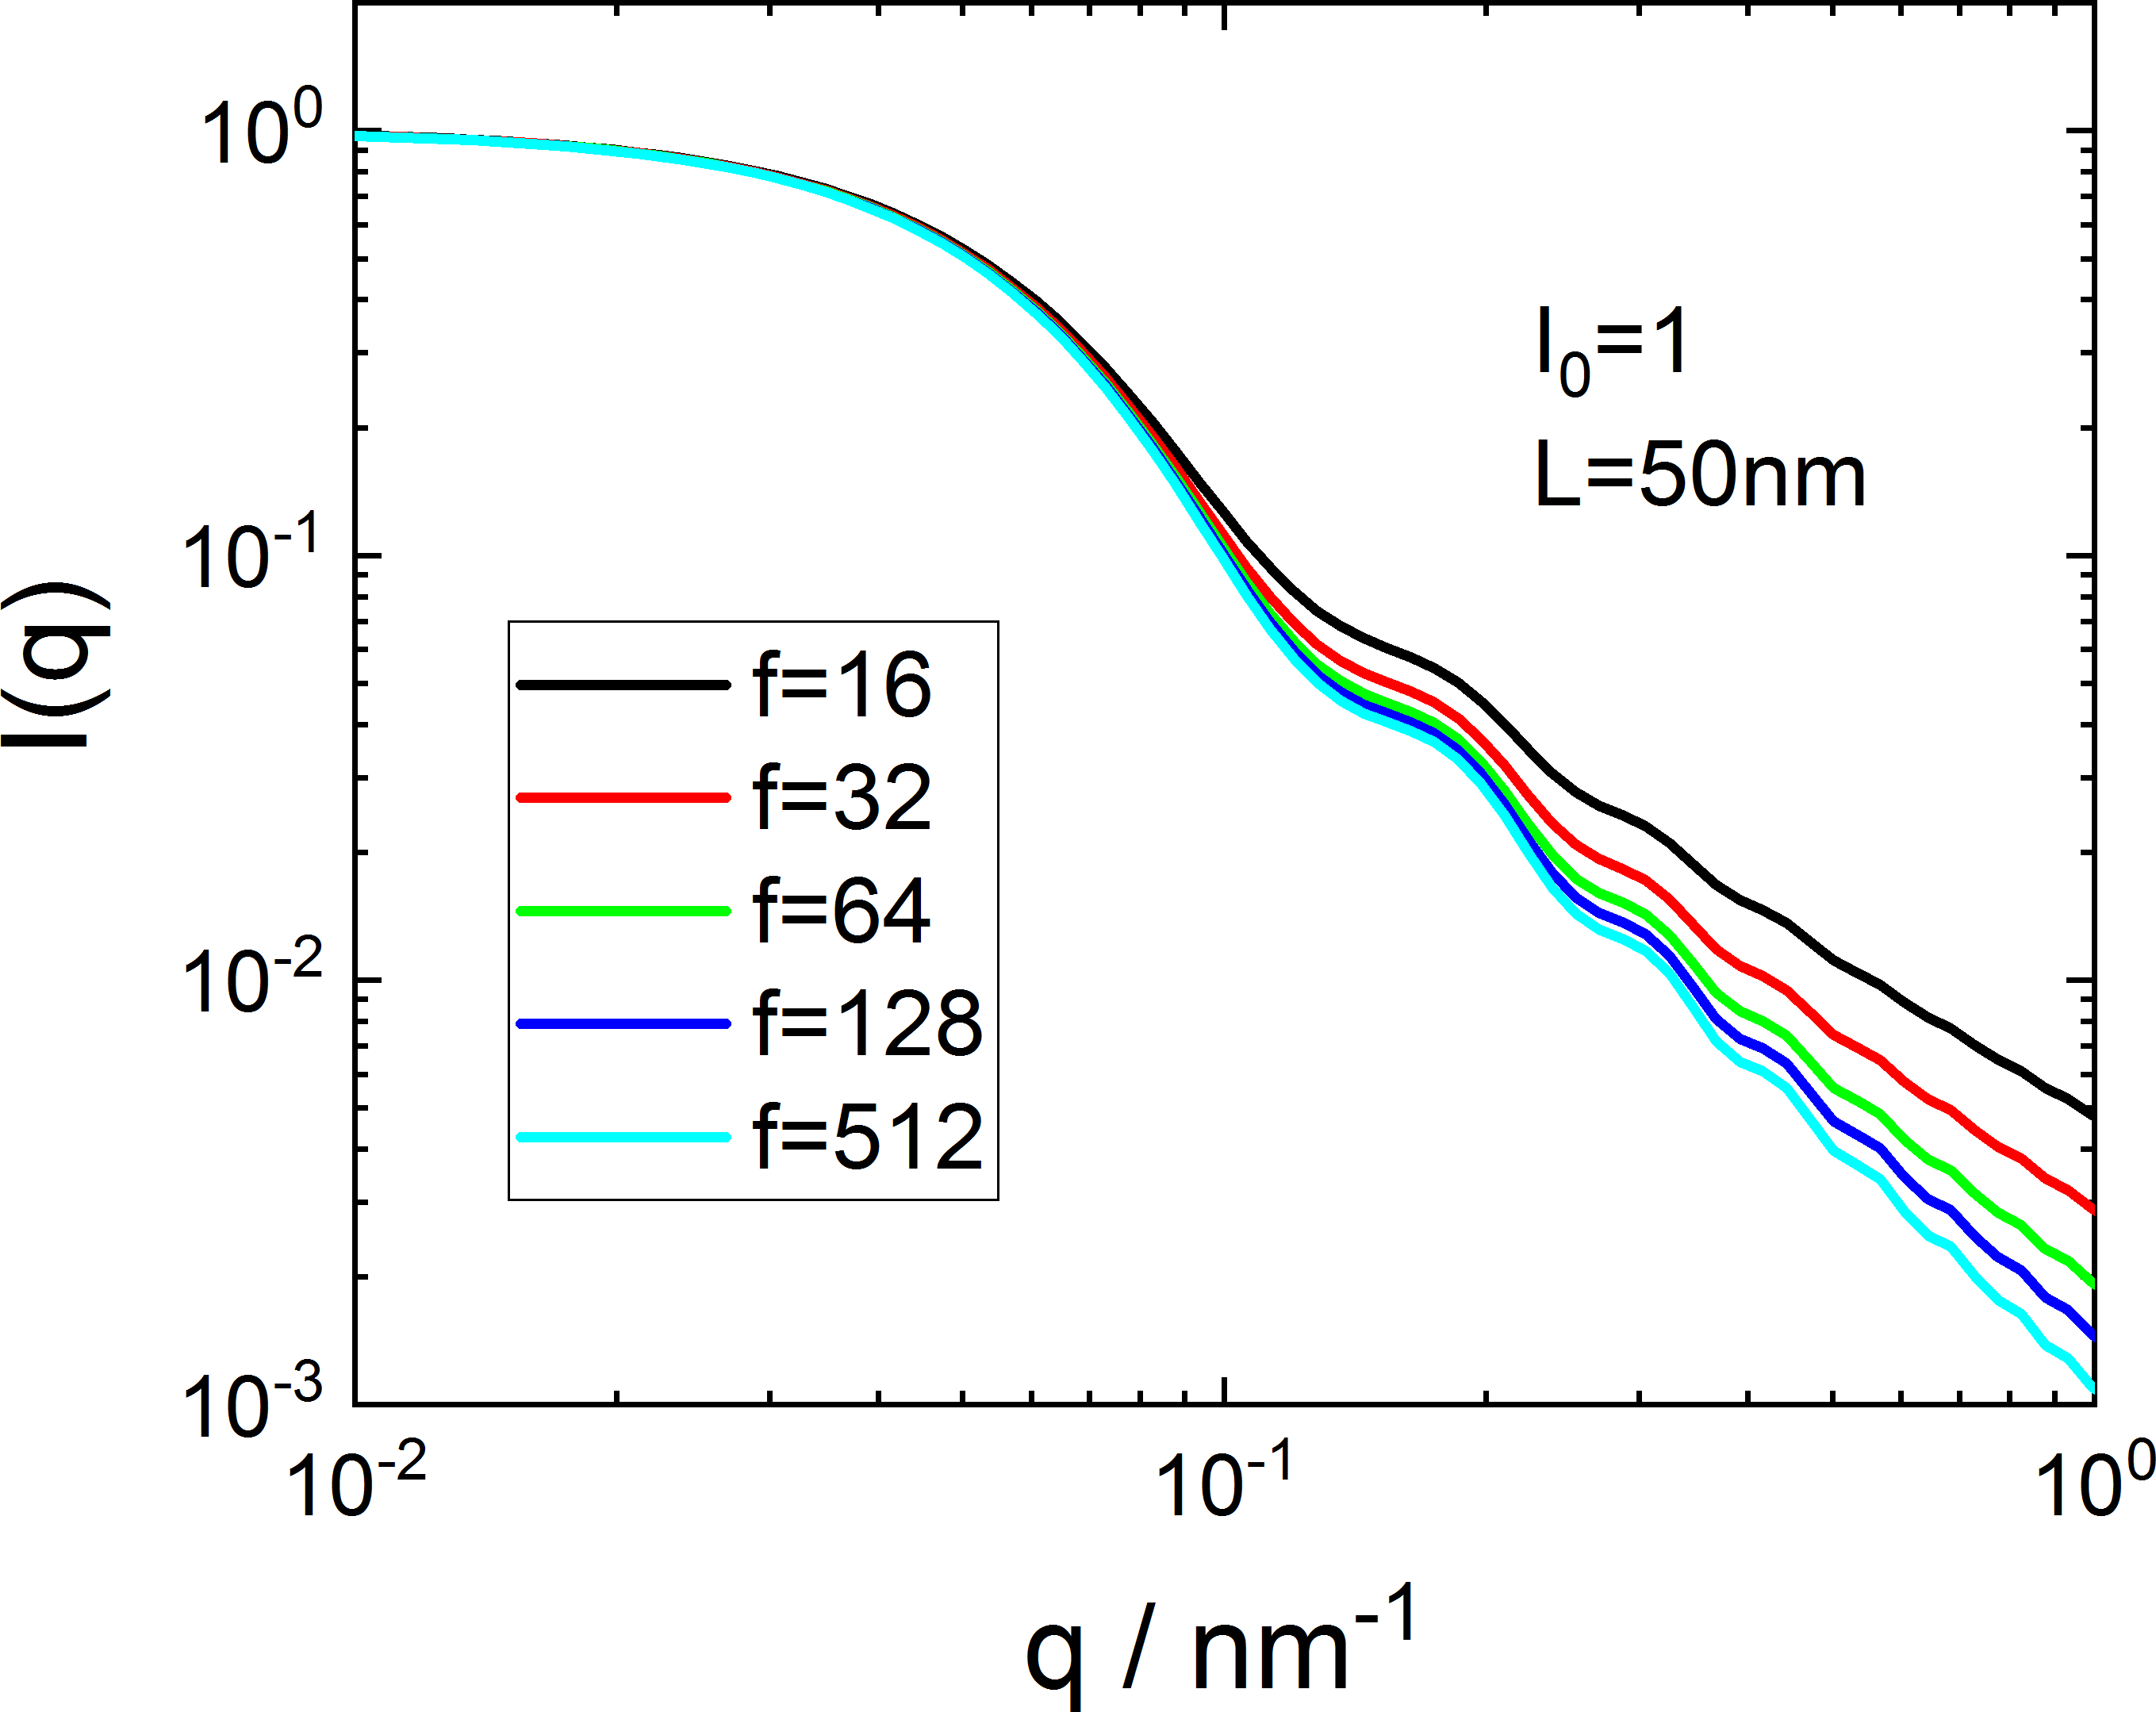
\includegraphics[width=0.75\textwidth]{../images/form_factor/stars/StarRigidRodsIQ.png}
\end{center}
\caption{Scattering function of a star polymer with arms of thin rigid rods.} \label{fig:StarRigidRods_Iq}
\end{figure}

\clearpage
\subsubsection{Star polymer with semi-flexible arms}
\label{sect:StarSemiflexible}~\\

\begin{figure}[htb]
\begin{center}
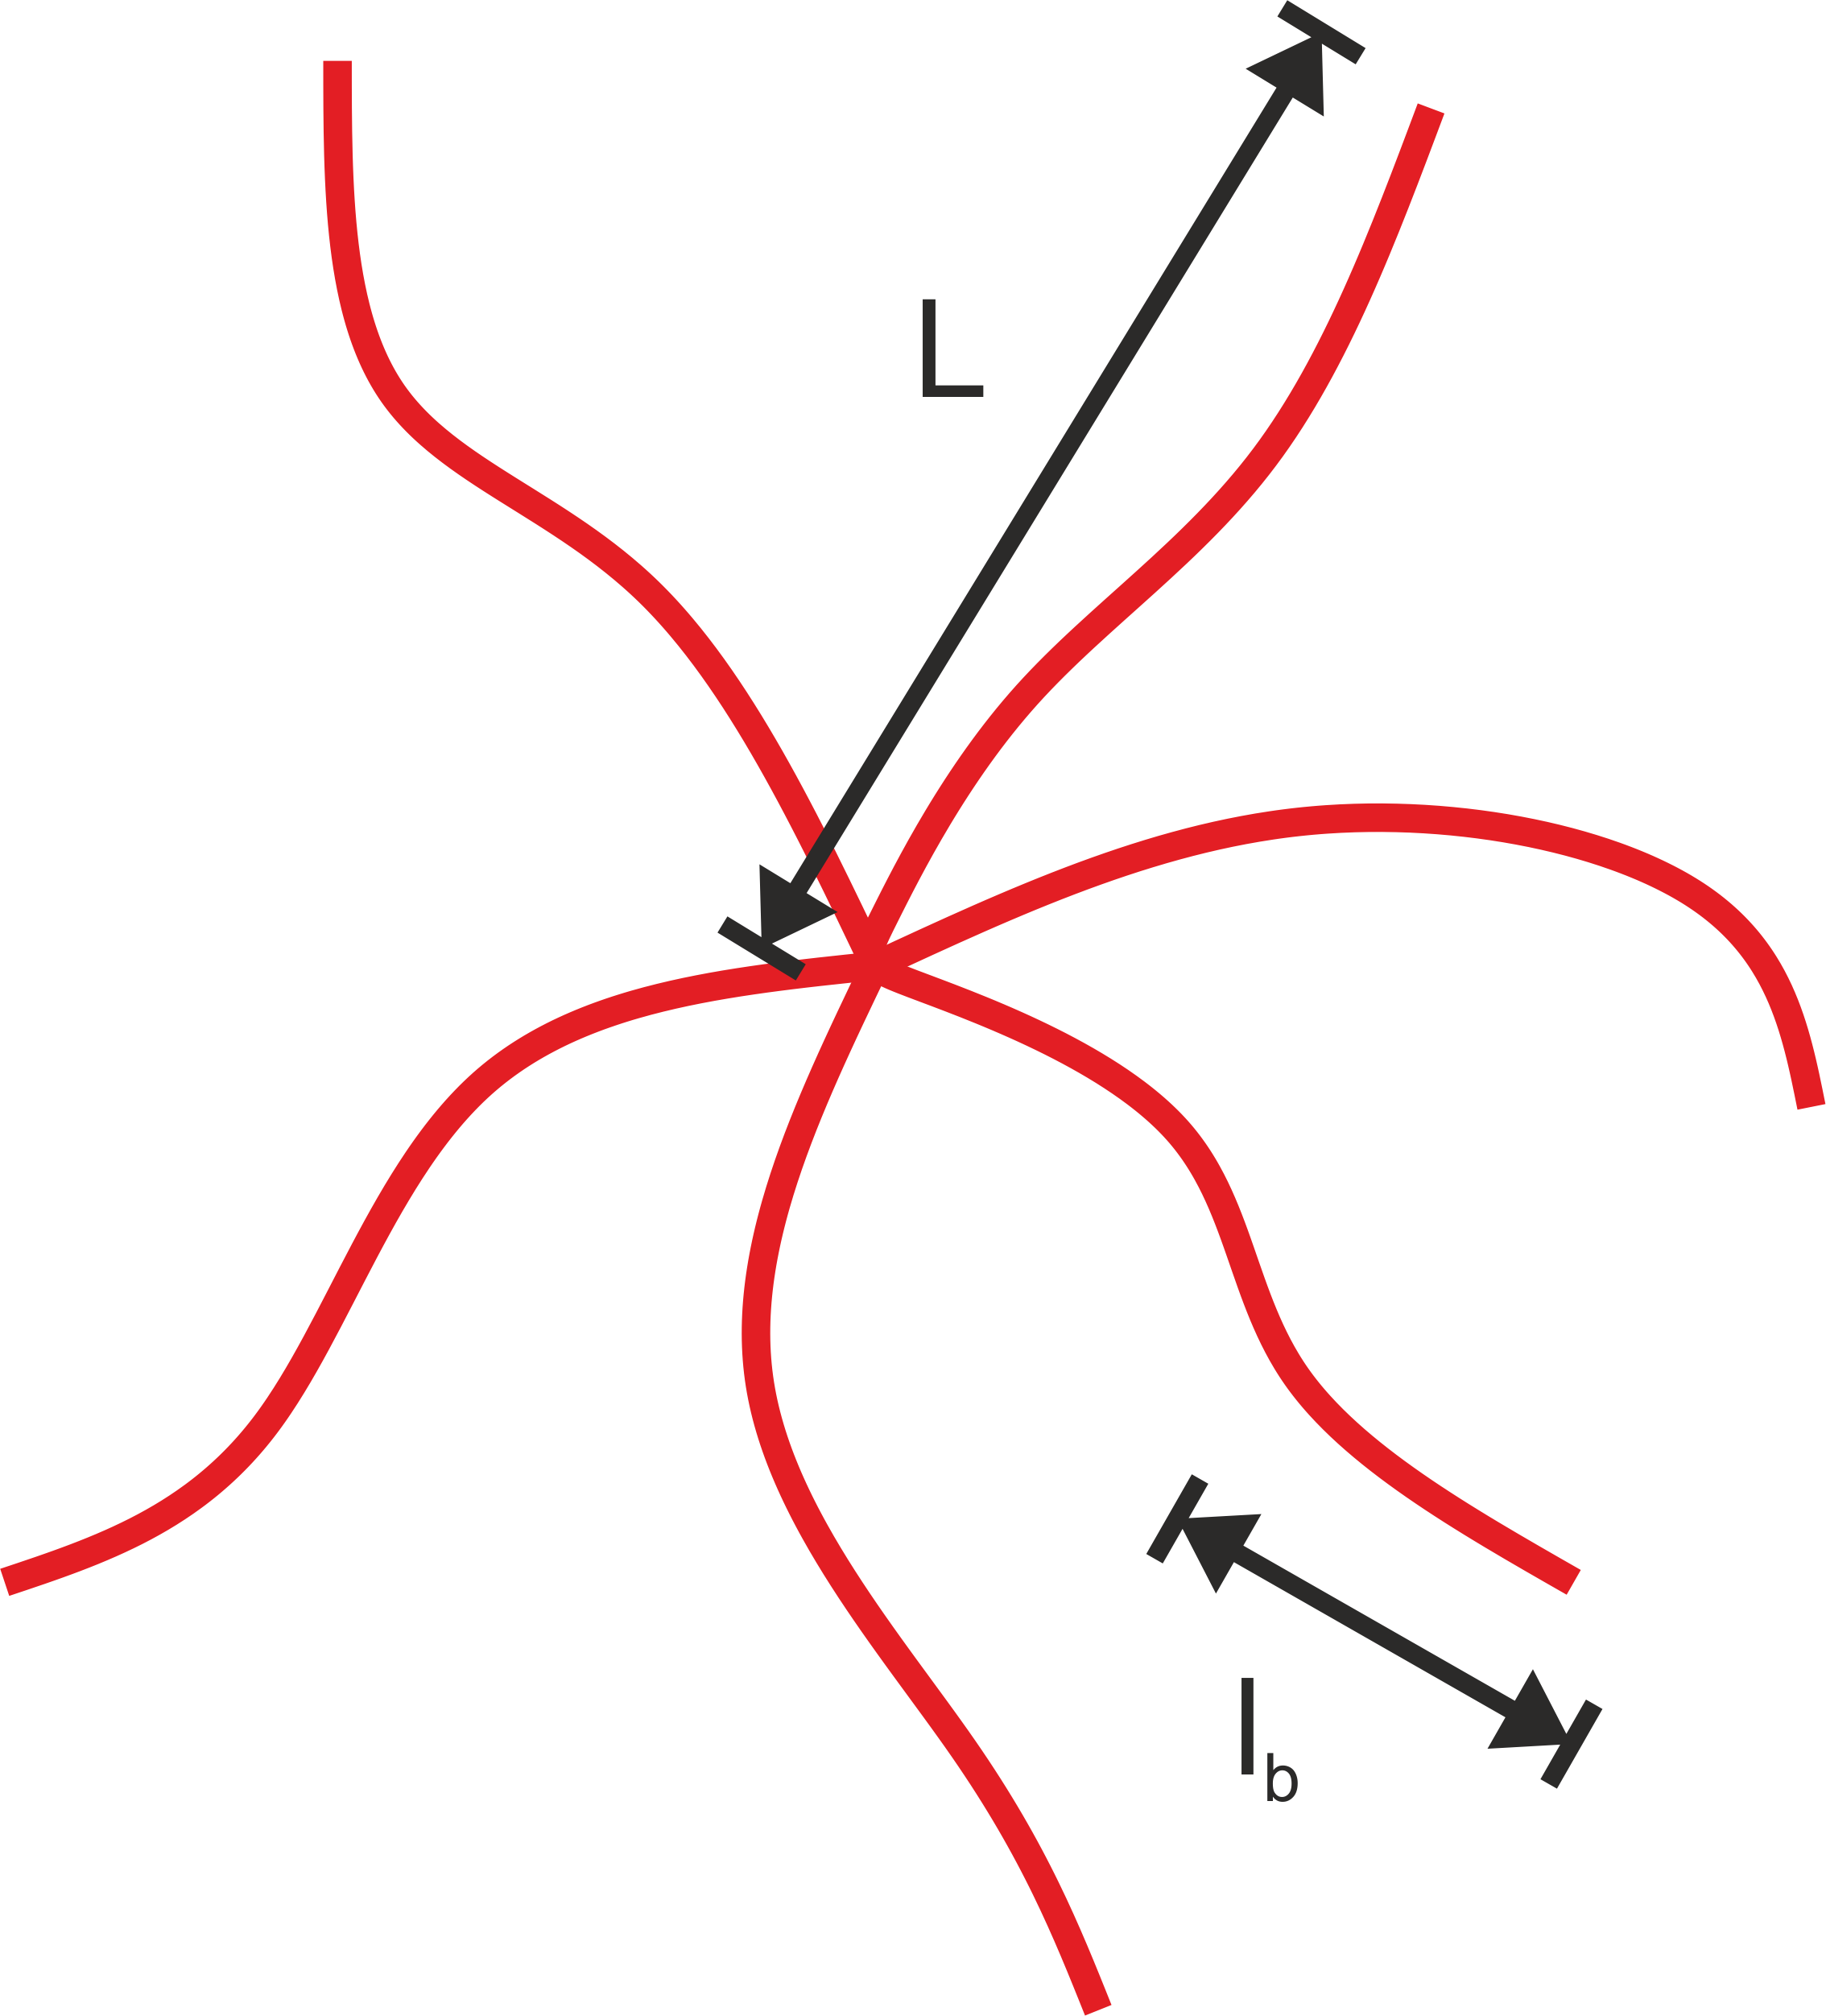
\includegraphics[width=0.4\textwidth]{semiflexiple_polymer_star.png}
\end{center}
\caption{Star with arms of semi-flexible (wormlike) polymers} \label{fig:semiflexiple_polymer_star}
\end{figure}

The derivation of the form factor of a star with semi-flexible arms can be found in \cite{Koyama1973,Koyama1974,Huber1989,Poetschke2000}. The resulting function for the
scattering intensity is given by
\begin{align}
 P_\mathrm{star}(Q) &= I_0/f\left(P_\mathrm{sb} + (f-1)P_\mathrm{ib} \right) \\
 P_\mathrm{sb} &= \frac{2}{X^2}\int_0^X (X-x)\phi(x)\mathrm{d}x \\
 P_\mathrm{ib} &= \left(\frac{1}{X}\int_0^X \phi(x)\mathrm{d}x\right)^2
\end{align}
with
\begin{align}
X &= \frac{2L}{l_b} \\
\phi(x) &= \exp\left(-\frac{s^2}{3}xf(x)\right) \frac{\sin(sxg(x))}{sxg(x)} \\
s &= \frac12 ql_b \\
xf(x) &= \frac{2\langle r^2\rangle}{l_b^2} - \frac12 x^2g^2(x) \\
x^2g^2(x) &= \frac{2\langle r^2\rangle}{l_b^2} \sqrt{10}\sqrt{1-\frac35 K}
\end{align}
and
\begin{align}
K &= \frac{\langle r^4\rangle}{\langle r^2\rangle^2} \\
\langle r^2\rangle &= \frac{l_b^2}{2} \left(x-\left(1-e^{-x}\right)\right)\\
\langle r^4\rangle &= \frac{l_b^4}{4} \left\{\frac53 x^2 -\frac{52}{9}x-\frac{2}{27}\left(1-e^{-3x}\right)+8\left(1-e^{-x}\right)-2xe^{-x}\right\}
\end{align}
The radius of gyration of a star polymer with semi-flexible arms is \cite{Mansfield1980,Huber1989}
\begin{align}
\begin{split}
R_\mathrm{G} &=
\Bigg[(3f - 2)\frac{2L}{3l_b} + 1 - 2f +
   \frac{l_b}{L} + 2(f - 1)\frac{l_b}{2L} x_1 \\
   & -2\left(\frac{l_b}{2L}\right)^2 x_1 + \left(1 - x_1\frac{l_b}{2L}\right)^2\Bigg]\frac{l_b^2}{4f}
\end{split} \\[3mm]
x_1 &= 1-\exp\left(-2L/l_b\right)
\end{align}
The limiting cases
\begin{align}
\lim_{l_b\to\infty} R_\mathrm{G} &= L^2/3 \\
\lim_{l_b\to 0} R_\mathrm{G} &= \frac{3f-2}{6f} Ll_b
\end{align}
correspond to the cases of a star with rigid rod and a star with Gaussian arms.

\vspace{5mm}

\noindent
\uline{Input Parameters for model \texttt{star polymer with semi-flexible arms}:}
\begin{description}
\item[\texttt{I0}] forward scattering $I_0$ for $q=0$
\item[\texttt{L}] contour length $L$ of a single arm
\item[\texttt{lb}] Kuhn length $l_b$ of the polymer arm
\item[\texttt{dummy}] not used
\item[\texttt{f}] number of arms $f$
\end{description}


\begin{figure}[htb]
\begin{center}
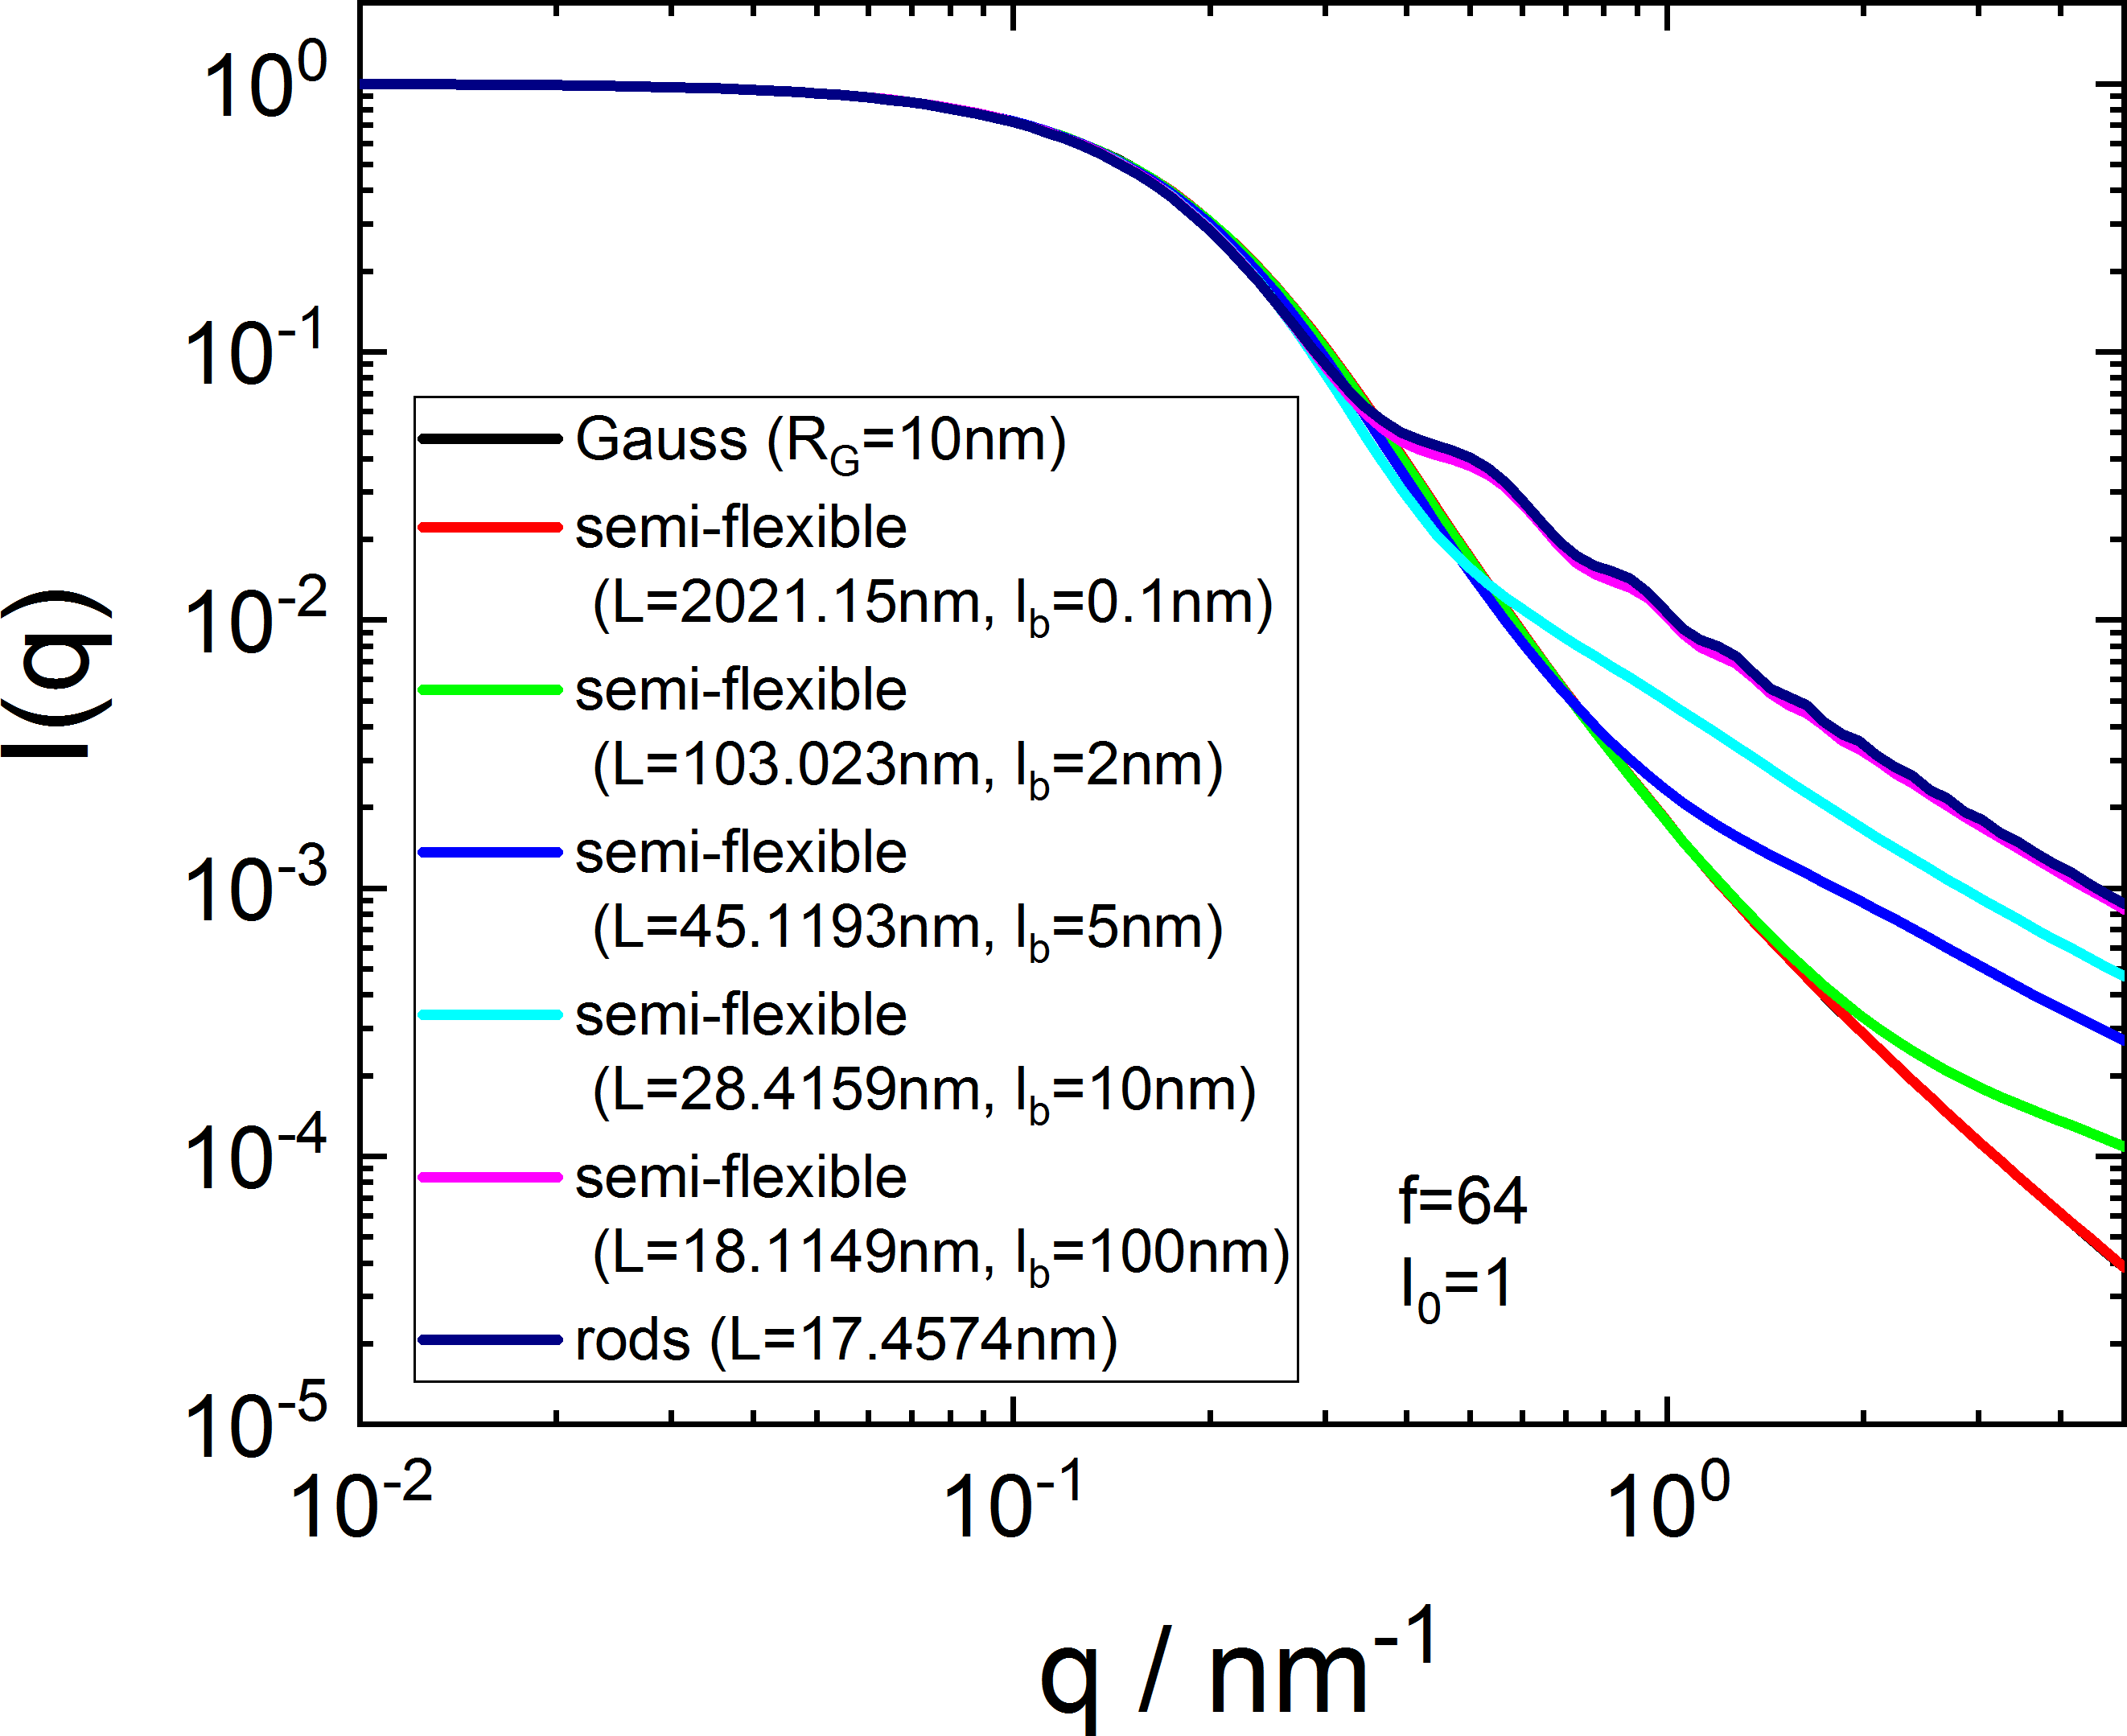
\includegraphics[width=0.75\textwidth]{../images/form_factor/stars/StarSemiFlexibleIQ.png}
\end{center}
\caption{Scattering function of a star polymer with semi-flexible arms. In the limit $l_b\rightarrow 0$ and $l_b\rightarrow 0$ the form factor is approximated by a star with gaussian arms and in stars with arms of rigid rods. The contour length $L$ and Kuhn length $l_b$ have been chosen to get always the same radius of gyration of 10nm.} \label{fig:StarSemiFlexible_Iq}
\end{figure}


\clearpage
\subsubsection{Star of gaussian polymer with excluded volume}
\label{sect:StarGaussianExvol}
~\\
In \cite{Hammouda2016} the star form factor including excluded volume effects takes the form factor of an individual polymer and combines it in terms of a combinatorial star according to \cite{Huber1989}. For this the form factor of a chain with the contour length $L$ of a single arm and that one with a contour length  of twice a single arm $2L$ is needed. As the Radius of gyration of a single arm scales according to eq.\ \ref{eq:Uexclvol} with $R_g \propto L^{2\nu}$ we get
\begin{align}
 P_\mathrm{star}(q) &= I_0/f\left(P_\mathrm{sb}(q,R_G) + (f-1)P_\mathrm{ib}(q,R_G) \right) \\
 P_\mathrm{sb}(q,R_G) &= \frac{1}{\nu U^{\frac{1}{2\nu}}}\gamma\left(\frac{1}{2\nu},U\right) -
 \frac{1}{\nu U^{\frac{1}{\nu}}}\gamma\left(\frac{1}{\nu},U\right)\\
 P_\mathrm{ib} &= 2P_\mathrm{sb}(q,2^{2\nu}R_G)-P_\mathrm{sb}(q,R_G)
\end{align}
with $\gamma(d,U)$ being the lower incomplete gamma-function and the definition of $U$ as
\begin{align}
\gamma(d,U) &= \int_0^U \exp(-t) t^{d-1}\mathrm{d}t \\
U &= q^2R_G^2\frac{(2\nu+1)(2\nu+2)}{6}
\end{align}

\vspace{5mm}

\noindent
\uline{Input Parameters for model \texttt{star of polymer arms with excl. vol.}:}
\begin{description}
\item[\texttt{I0}] forward scattering $I_0$ for $q=0$
\item[\texttt{Rg}] radius of gyration $R_G$ of a single arm
\item[\texttt{nu}] Flory exponent $\nu$ of the polymer arm
\item[\texttt{dummy}] not used
\item[\texttt{f}] number of arms $f$
\end{description}


\begin{figure}[htb]
\begin{center}
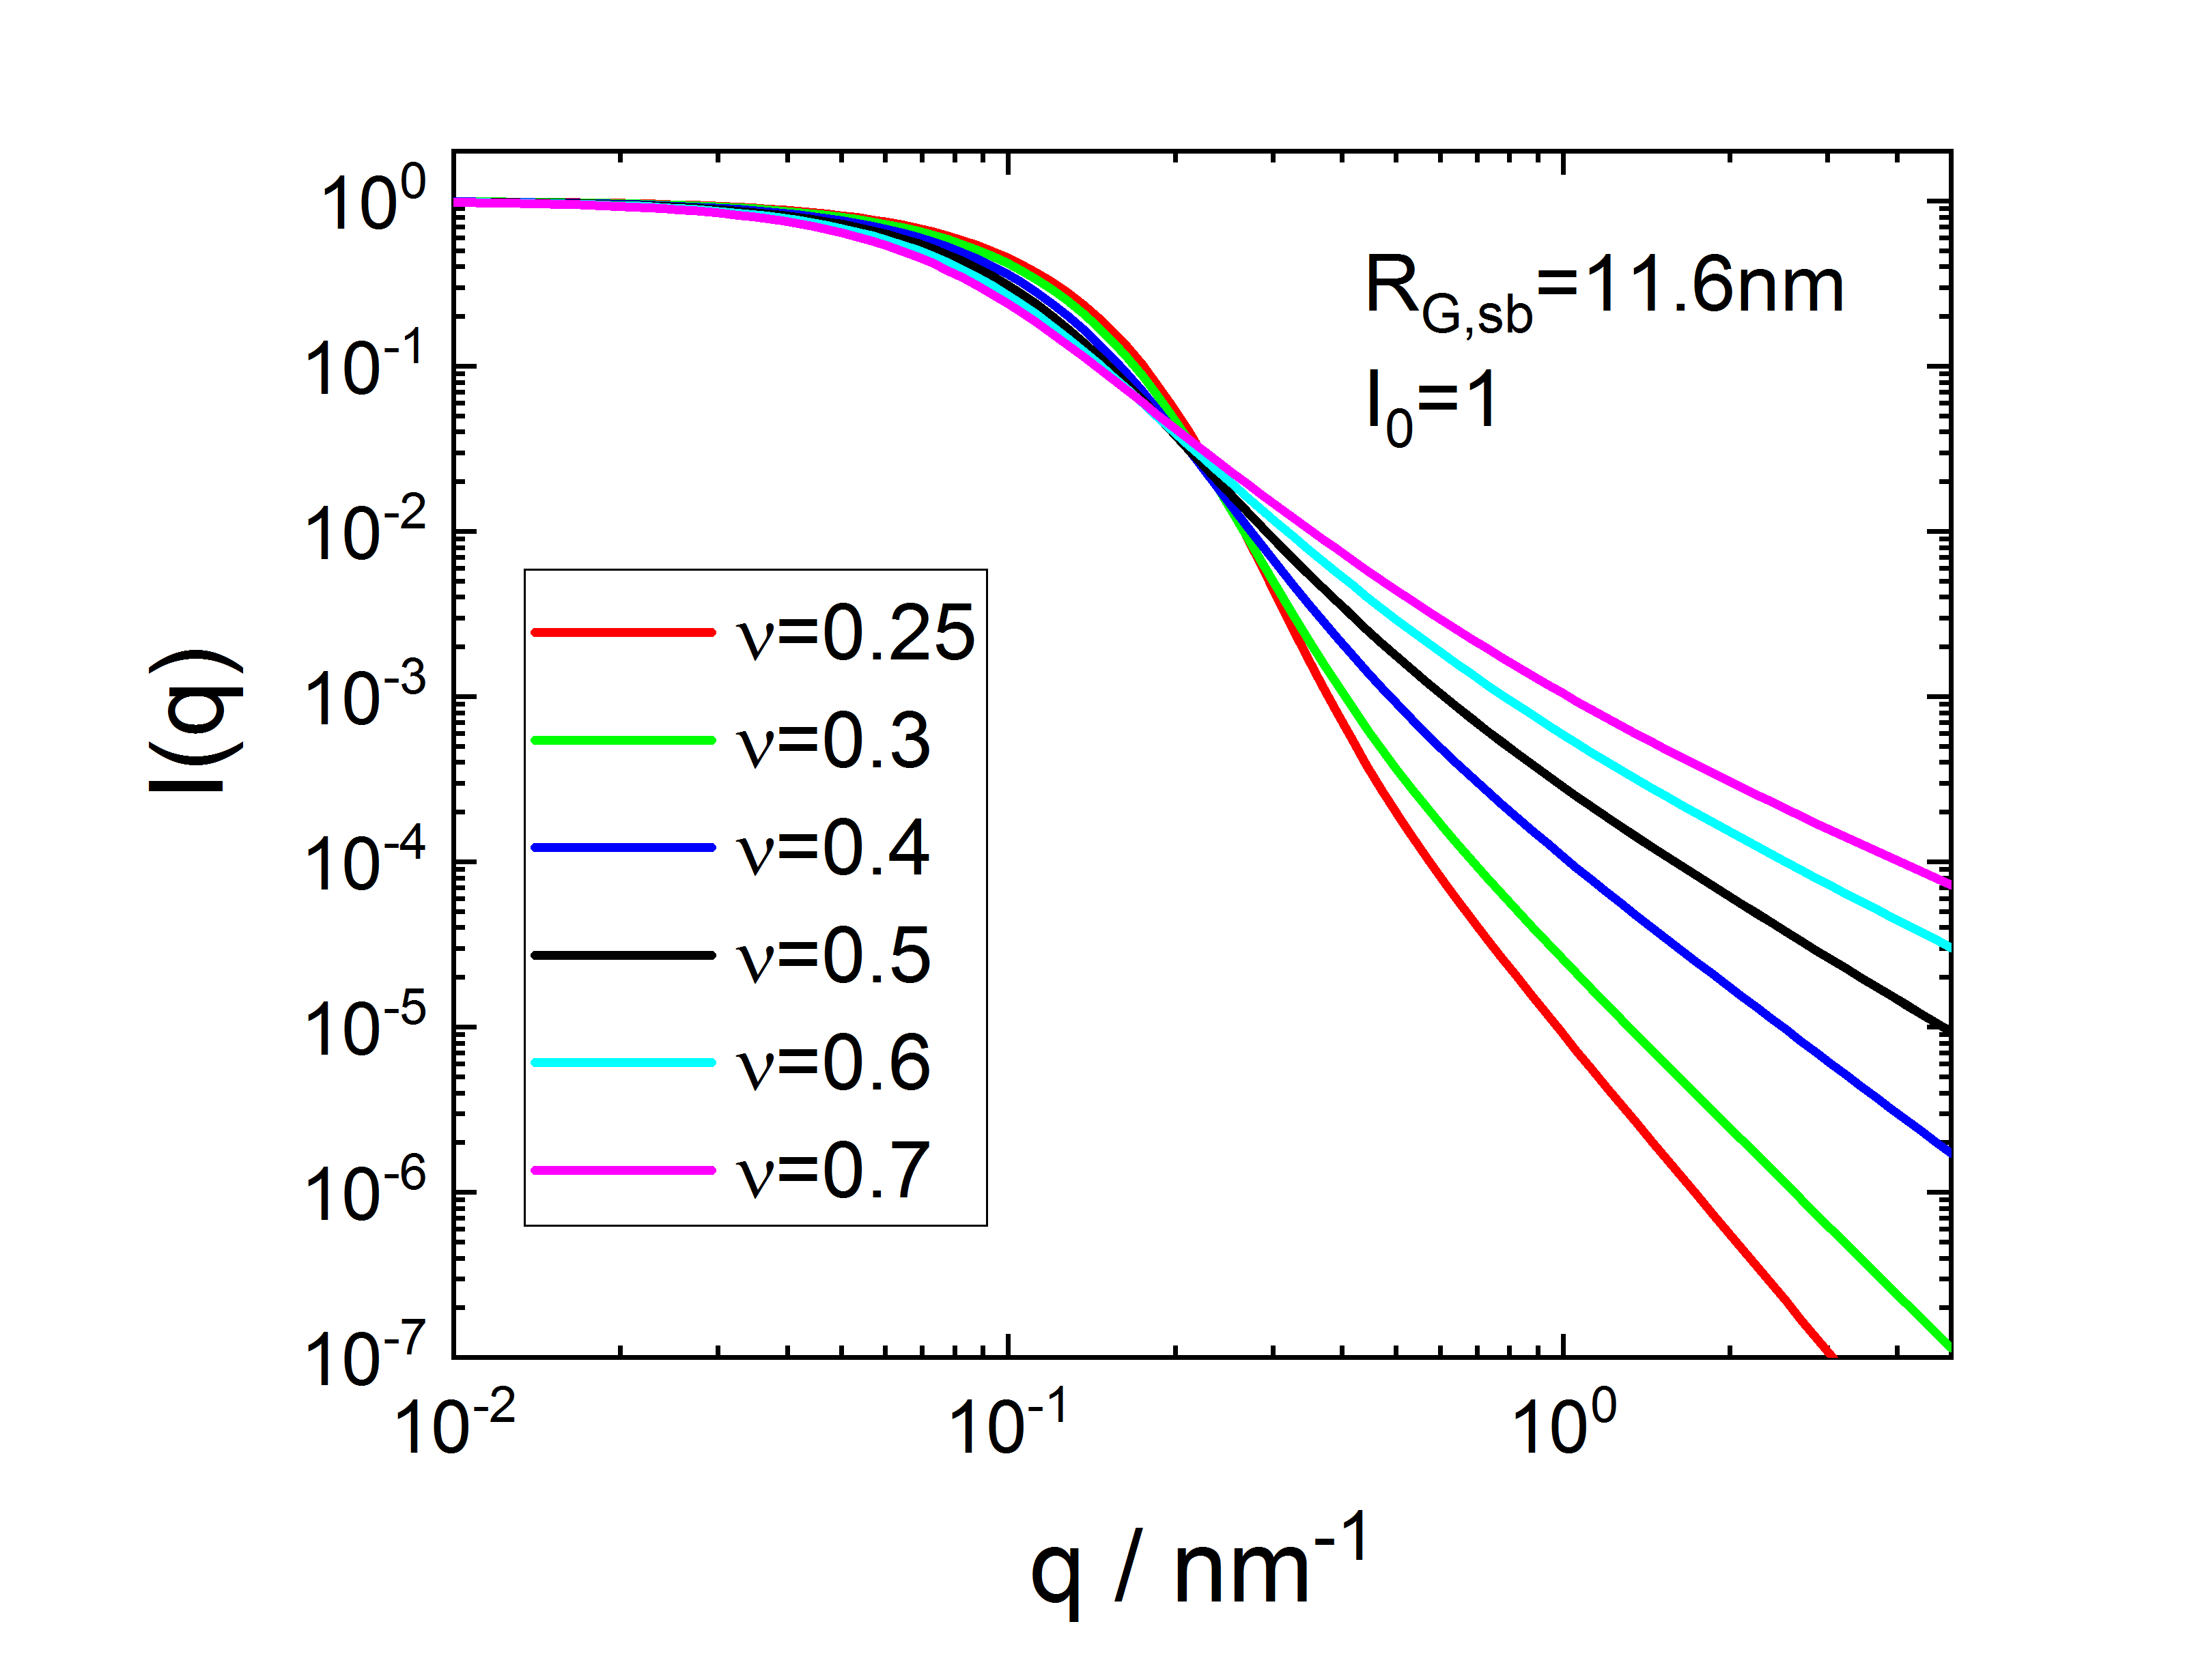
\includegraphics[width=0.75\textwidth]{../images/form_factor/stars/StarGaussExclVolIQ.png}
\end{center}
\caption{Scattering function of a star polymer with arms following Gaussian statistics with excluded volume effects. For $\nu=1/2$ the scattering curves is identical to the \texttt{BenoitStar}. } \label{fig:StarSemiFlexible_Iq}
\end{figure}


%%%%%%%%%%%%%%%%%%%%%%%%%%%%%%%%%%%%%%%%%%%%%%%%%%%%%%%%%%%%%%%%%%%%%
\clearpage
\subsubsection{Polydisperse star polymer with Gaussian statistics \cite{Burchard1974}}
\label{sect:PolydisperseStar}
~\\
\begin{figure}[htb]
\begin{center}
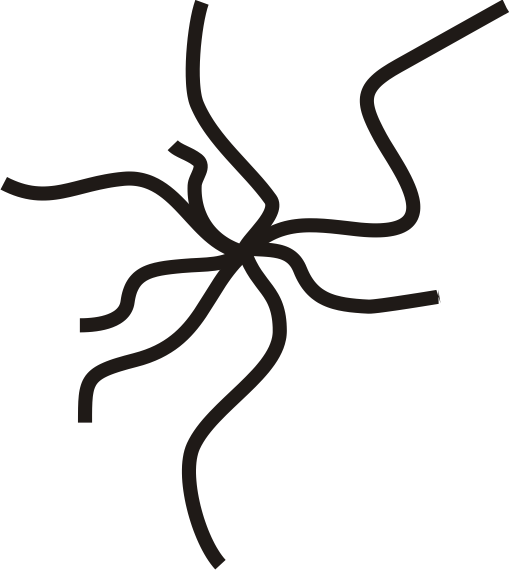
\includegraphics[width=0.2545\textwidth,height=0.2535\textwidth]{polyBenoit.png}
\end{center}
\caption{Polydisperse star polymer with Gaussian statistics} \label{fig:polyBenoitStar}
\end{figure}

For a Schulz–Flory (most probable) distribution (Schulz–Zimm distribution
with $z = 1$) for the mass distribution of the arms, Burchard \cite{Burchard1974} has given the form factor:
\begin{align}
I_\text{PolydisperseStar}(Q) &= I_0
\frac{1+\frac{u^2}{3 f}}{\left(1+\frac{u^2(f +1)}{6 f }\right)^2}
\end{align}
where $f$ is the number of arms and $u^2 = \langle R_g^2 \rangle_z \,Q^2$, where
$\langle R_g^2 \rangle_z$ is the $z$-average radius of gyration squared of an arm.

\vspace{5mm}

\noindent
\uline{Input Parameters for model \texttt{PolydisperseStar}:}
\begin{description}
\item[\texttt{I0}] forward scattering $I_0$
\item[\texttt{R\_G}] radius of gyration $R_G$
\item[\texttt{dummy}] not used
\item[\texttt{dummy}] not used
\item[\texttt{f}] number of arms $f$
\end{description}


\begin{figure}[htb]
\begin{center}
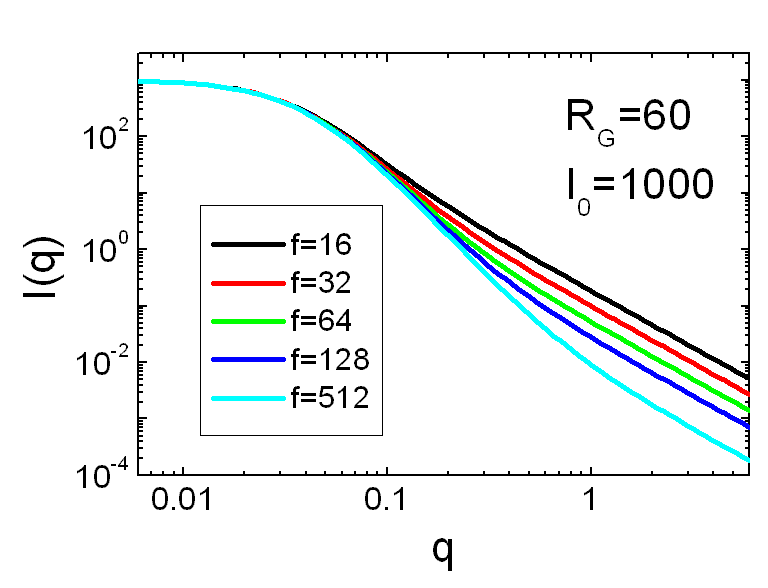
\includegraphics[width=0.768\textwidth,height=0.588\textwidth]{polyBenoit_Iq.png}
\end{center}
\caption{Scattering function of a polydisperse star polymer with Gaussian statistics.} \label{fig:polyBenoit_Iq}
\end{figure}



%%%%%%%%%%%%%%%%%%%%%%%%%%%%%%%%%%%%%%%%%%%%%%%%%%%%%%%%%%%%%%%%%%%%%%%%%%%%%%%%%%%%%%%%
\clearpage
\subsubsection{Star polymer according to Dozier}
\label{sect:DozierStar}
~\\
\subsubsection{Dozier}
\label{sect:DozierStar1}
~\\
\begin{figure}[htb]
\begin{center}
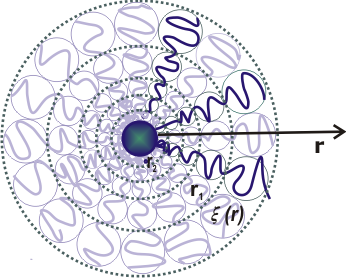
\includegraphics[width=0.346\textwidth,height=0.278\textwidth]{Dozier.png}
\end{center}
\caption{Star polymer according to Dozier} \label{fig:DozierStar}
\end{figure}
Branched polymers having all branches emanating from
the center of the macromolecule are commonly called star
polymers. For a star polymer Dozier \cite{dozier91} has developed
a scattering function which reads:
\begin{align}
I_\text{DozierStar}(Q,I_0,R_G,\alpha,\nu,f)
& = I_0 \exp\left(-\frac{Q^2R_G^2}{3}\right) \\
+& \frac{4\pi\alpha}{Q\xi} \Gamma(\mu)
\frac{\sin(\mu\arctan(Q\xi))}{(1+Q^2\xi^2)^{\mu/2}} \nonumber
\end{align}
with $\mu=1/\nu-1$ and $\xi=2R_G/\sqrt{f}$.
\begin{align}
I_0      & : \text{scale parameter} \nonumber \\
R_G      & : \text{radius of gyration} \nonumber \\
\alpha   & : \text{scale parameter for fractal term} \nonumber \\
\nu      & : \text{Flory exponent, 3/5 in good solvent, 1/2 in $\Theta$-solvent} \nonumber \\
f        & : \text{number of arms in the star} \nonumber
\end{align}

\vspace{5mm}

\noindent
\uline{Input Parameters for model \texttt{Dozier}:}
\begin{description}
\item[\texttt{I\_0}] scale parameter if the Gaussian term $I_0$
\item[\texttt{R\_G}] radius of gyration $R_G$
\item[\texttt{alpha}] scale parameter for fractal term $\alpha$
\item[\texttt{nu}] excluded volume parameter or Flory exponent $\nu$
\item[\texttt{f}]  number of arms $f$ in the star
\end{description}
\vspace{5mm}

\begin{figure}[htb]
\begin{center}
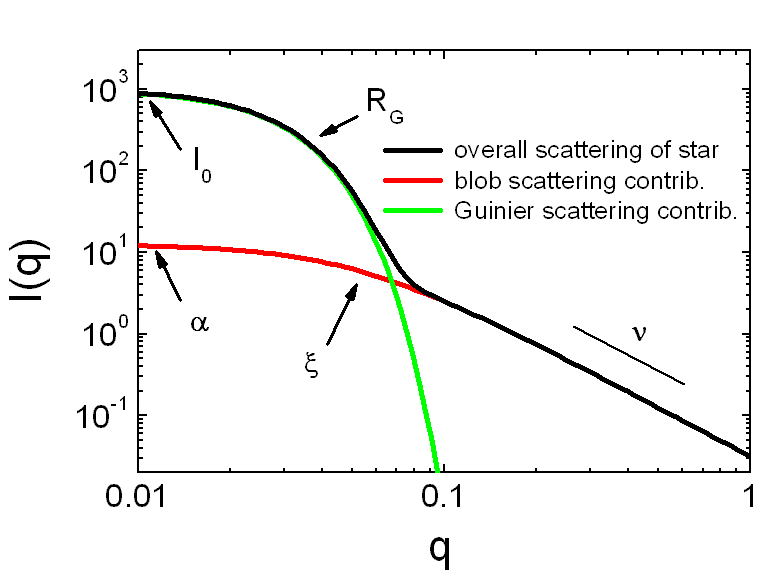
\includegraphics[width=0.768\textwidth,height=0.588\textwidth]{Dozier_Iq.png}
\end{center}
\caption{Scattering function of a star polymer according to Dozier: $I0=10^3$, $R_g=60$, $\alpha=1$
$\xi=20$, $\nu=1/2$ } \label{fig:IQDozierStar1}
\end{figure}

\clearpage
\subsubsection{Dozier2}
\label{sect:DozierStar2}
~\\
This is a re-parametrization of the \texttt{Dozier} form factor
to scale the scattering of the overall star to the local scattering of the individual arms.
\begin{align}
I_\text{DozierStar2}(Q,I_0,R_G,f,\nu)=
\frac{I_0}{f}
\Biggl(
 &  (f-1)
    \exp\left(-\frac{Q^2R_G^2}{3}\right) \\
 +&  \frac{\Gamma(\mu)}{Q\xi}
    \frac{\sin(\mu\arctan(Q\xi))}{(1+Q^2\xi^2)^{\mu/2}} \nonumber
\Biggr)
\end{align}
with $\mu=1/\nu-1$ and $\xi=2R_G/\sqrt{f}$.
\begin{align}
I_0      & : \text{scale parameter} \nonumber \\
R_G      & : \text{radius of gyration of the star} \nonumber \\
\xi      & : \text{exponential damping length in mass fractal } \xi=2R_G/\sqrt{f}\nonumber \\
\nu      & : \text{Flory exponent, 3/5 in good solvent, 1/2 in $\Theta$-solvent} \nonumber \\
f & : \text{number of arms in the star} \nonumber \\
\end{align}

\vspace{5mm}

\noindent
\uline{Input Parameters for model \texttt{Dozier2}:}
\begin{description}
\item[\texttt{I\_0}] scale parameter $I_0$
\item[\texttt{R\_G}] radius of gyration of the star $R_G$
\item[\texttt{dummy}] not used
\item[\texttt{nu}] Flory exponent, $\nu=3/5$ in good solvent, $\nu=1/2$ in $\Theta$-solvent
\item[\texttt{f}]  number of arms $f$ in the star from which the scale parameter for the fractal term is calculated.
\end{description}
\vspace{5mm}

\begin{figure}[htb]
\begin{center}
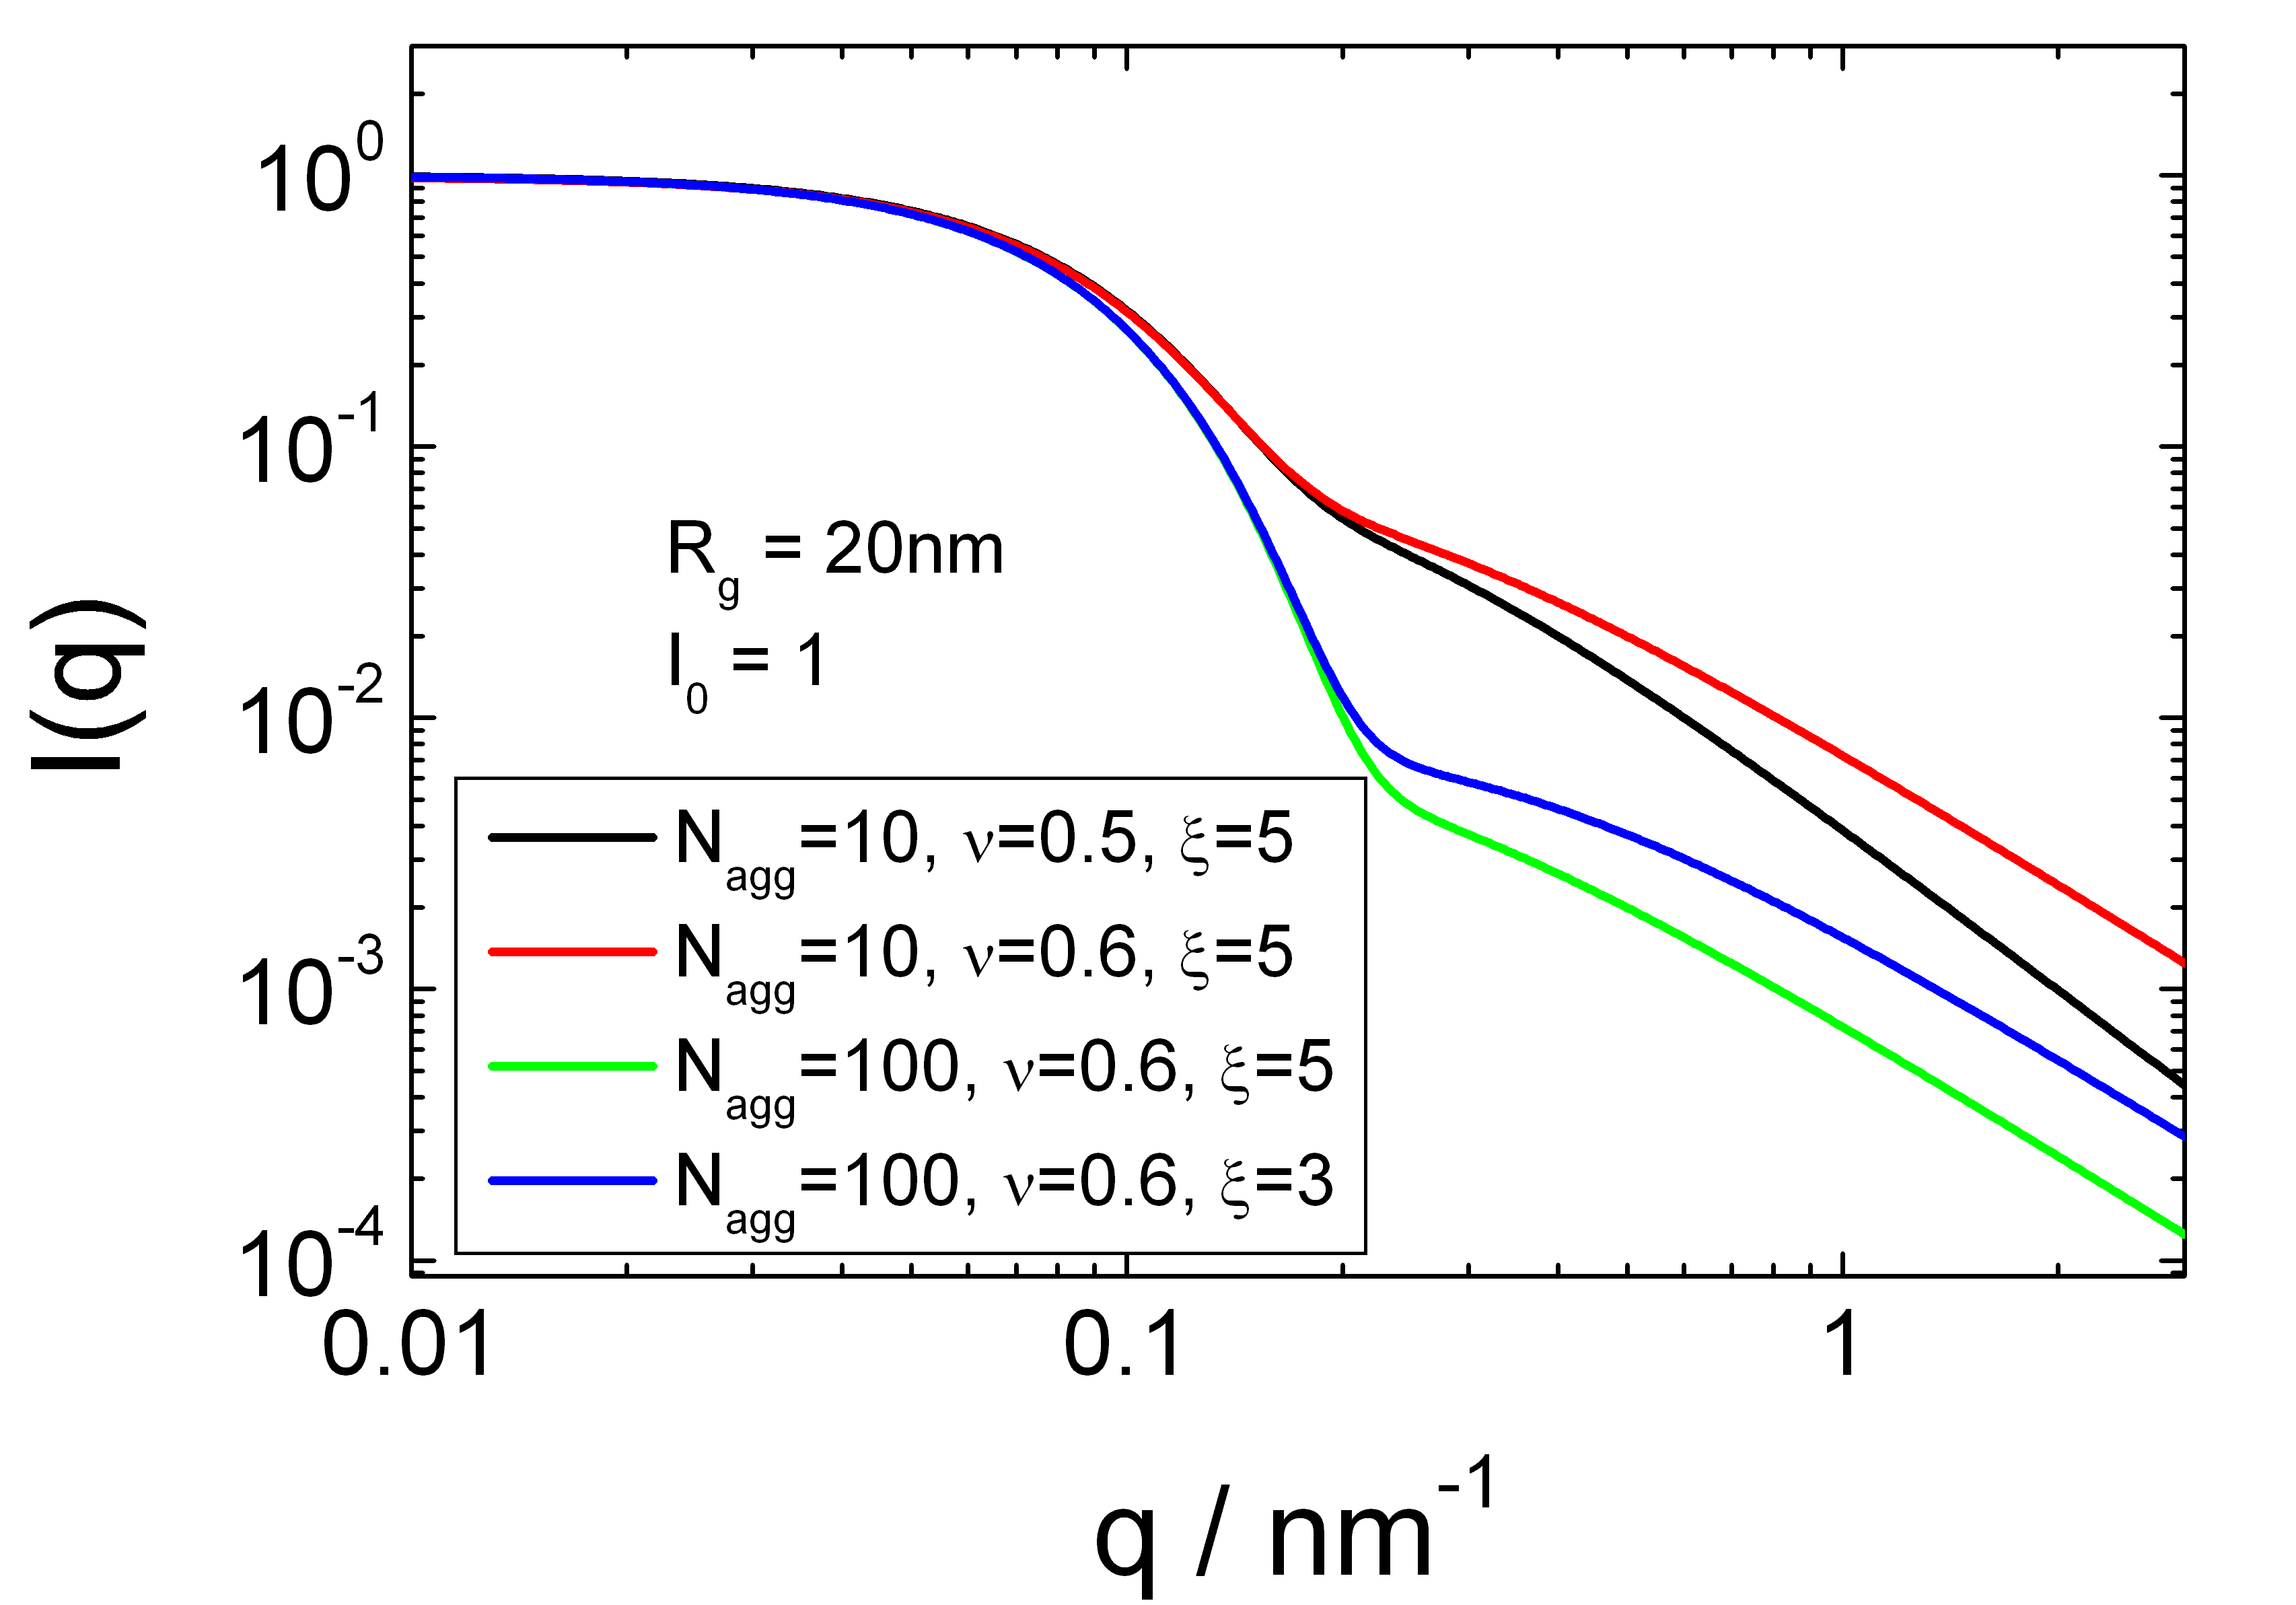
\includegraphics[width=0.768\textwidth,height=0.588\textwidth]{Dozier2_Iq.png}
\end{center}
\caption{Scattering function of a star polymer according to Dozier but modified
to scale the scattering of the overall star to the local scattering of the individual arms
by the number of arms} \label{fig:IQDozierStar2}
\end{figure}
\clearpage
%%%%%%%%%%%%%%%%%%%%%%%%%%%%%%%%%%%%%%%%%%%%%%%%%%%%%%%%%%%%%%%%%%%%%%%%

\subsection{Ring Polymers}
\subsubsection{Flexible Ring Polymer }
\label{sect:FlexibleRingPolymer}
~\\
Three different versions of a ring polymer have been implemented. The form factor of a cyclic chain under theta solvent conditions was first calculated by Casassa
using the Gaussian approximation \cite{Casassa1965,Burchard1996}. The formalism has been extended to ring polymers with an excluded volume parameter or Flory parameter $\nu$ \cite{Bensafi2000,Goosen2015}.

The classical form factor of Casassa for a flexible ring polymer following Gaussian statistics in a theta solvent is given by
\begin{figure}[htb]
\begin{center}
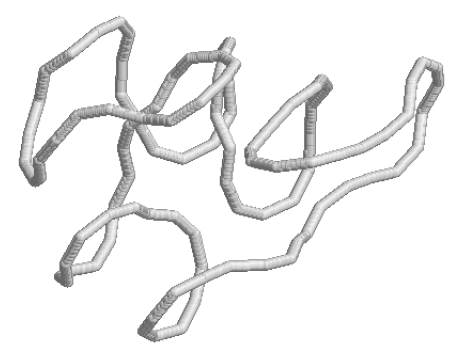
\includegraphics[width=0.471\textwidth,height=0.353\textwidth]{flexibleRing.png}
\end{center}
\caption{Sketch of a flexible ring polymer.}
\label{fig:flexibleRing}
\end{figure}

\begin{align}\label{eq:rinpolymerCasassa}
P_{1r}(q) & = \sqrt{\frac{2}{u_{1r}^2}} D\left[ \sqrt{\frac{u_{1r}^2}{2}} \right] \\
u_{1r}^2 &= q^2R^2_{g,1r} \\
R^2_{g,1r} &= \frac{b^2N}{12} \\
D(X) &= \exp\left(X^2\right) \int_0^X \exp(t^2)\, \mathrm{d}t
\end{align}

For ring polymers in a poor or very good solvent show excluded volume effects for which Bloomfeld and Zimm \cite{Bloomfield1966,Bensafi2000,Goosen2015} have calculated the radius of gyration. The corresponding scattering function can be found in \cite{Bensafi2000}.
\begin{align}\label{eq:rinpolymerBZ}
  P_{BZ,1r}(q) &= 2   \int_{0}^{1}(1-x)\exp\left(-\mu\frac{(1-x)^{1+\epsilon}x^{1+\epsilon}}{(1-x)^{1+\epsilon}+x^{1+\epsilon}}\right)\mathrm{d}x \\
  \mu &= \frac{q^2 R^2_{g,1r}}{6 K_{BZ}} \\
  K_{BZ} &= \int_0^1 \frac{(1-X)^{2+\epsilon}X^{1+\epsilon}}{(1-X)^{1+\epsilon}+X^{1+\epsilon}}\mathrm{d}X \\
  \epsilon &= 2\nu-1
\end{align}


Bensafi et al.\  \cite{Bensafi2000} also have given a semi-empirical description of a ring polymer with excluded volume effects
\begin{align}\label{eq:rinpolymerBMB}
  P_{BMP,1r}(q) &= 2 \int_{0}^{1}(1-x)\exp\left(-\mu (1-x)^{1+\epsilon}x^{1+\epsilon}\right)\mathrm{d}x \\
  \mu &= \frac{q^2 R^2_{g,1r}}{6 K_{BMB}} \\
  K_{BMB} &= \int_0^1 (1-X)^{2+\epsilon}X^{1+\epsilon} \mathrm{d}X \\
  \epsilon &= 2\nu-1
\end{align}

\vspace{5mm}

\noindent
\uline{Input Parameters for model \texttt{RingPolymerCasassa}:}
\begin{description}
\item[\texttt{Rg}] radius of gyration $R_G$
\item[\texttt{dummy}] not used
\item[\texttt{dummy}] not used
\item[\texttt{I0}] forward scattering $I_0$
\end{description}

\noindent
\uline{Input Parameters for model \texttt{RingPolymerBZ}:}
\begin{description}
\item[\texttt{Rg}] radius of gyration $R_G$
\item[\texttt{dummy}] not used
\item[\texttt{nu}] excluded volume parameter
\item[\texttt{I0}] forward scattering $I_0$
\end{description}

\noindent
\uline{Input Parameters for model \texttt{RingPolymerBMB}:}
\begin{description}
\item[\texttt{Rg}] radius of gyration $R_G$
\item[\texttt{dummy}] not used
\item[\texttt{nu}] excluded volume parameter
\item[\texttt{I0}] forward scattering $I_0$
\end{description}

\begin{figure}[htb]
\begin{center}
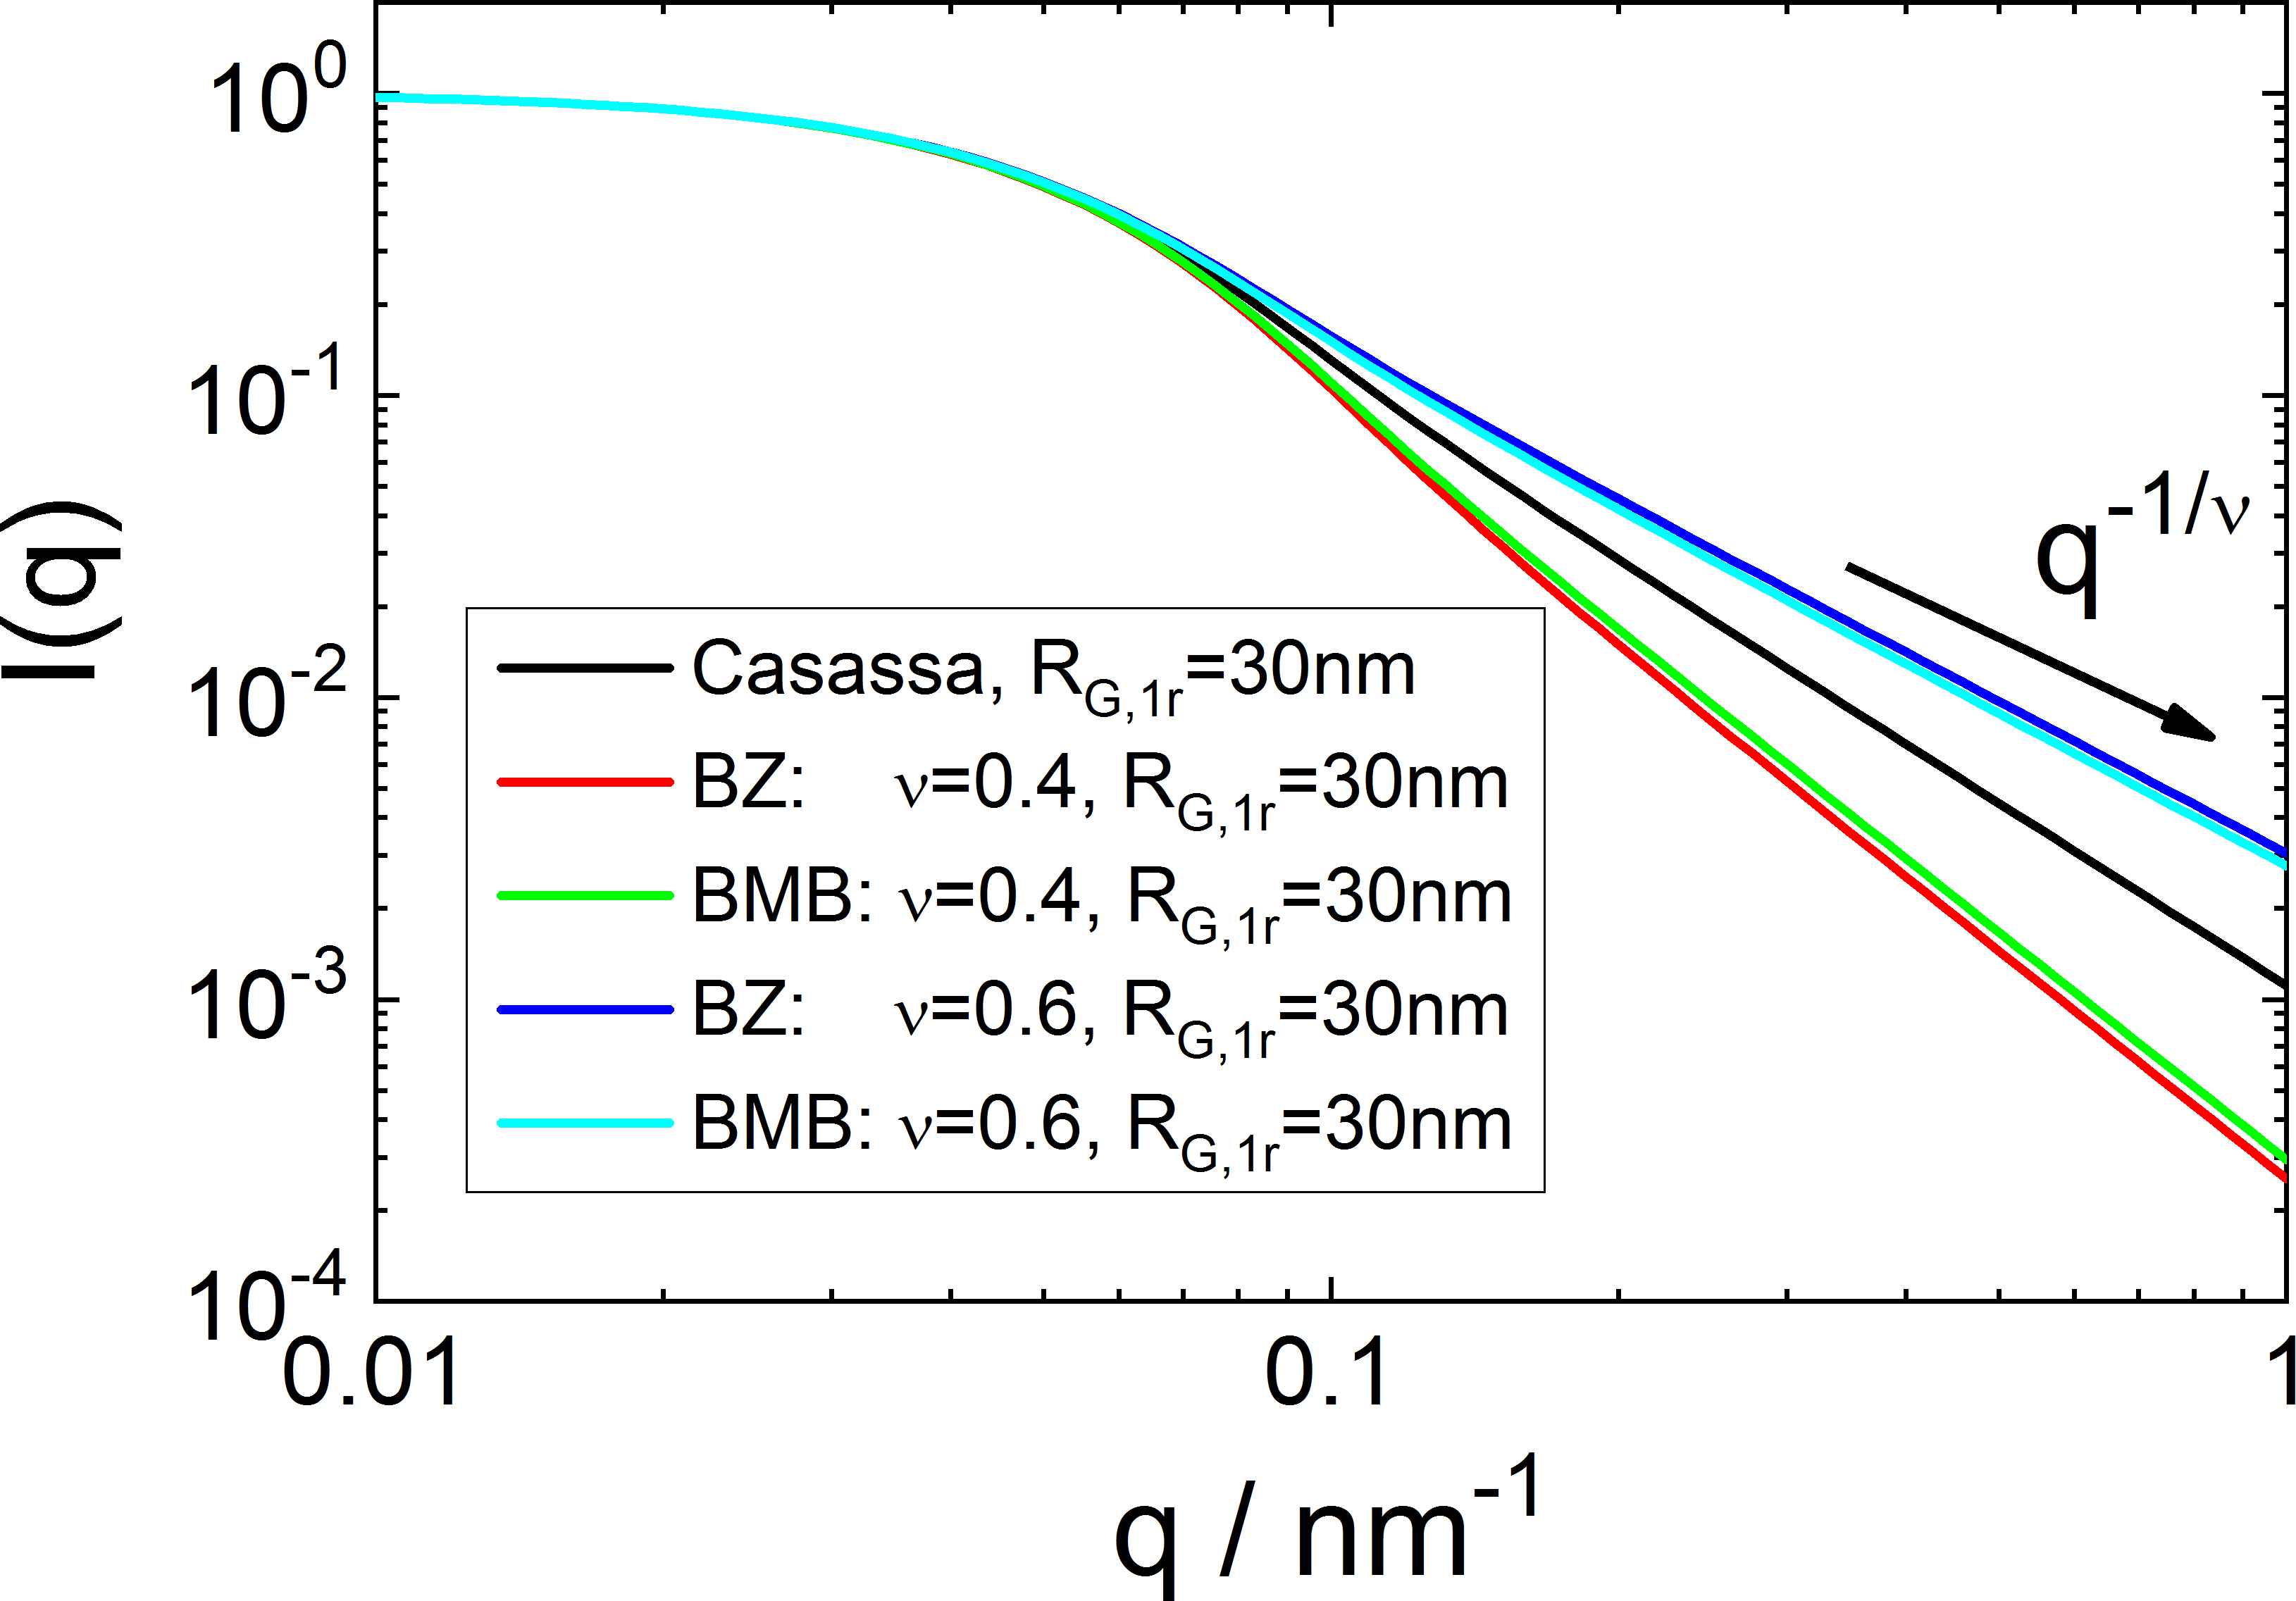
\includegraphics[width=0.768\textwidth]{../images/form_factor/polymer_rings/ringIQ.png}
\end{center}
\caption{Scattering intensity of ring polymers of different radius of gyration.} \label{fig:ringIQ}
\end{figure}

%%%%%%%%%%%%%%%%%%%%%%%%%%%%%%%%%%%%%%%%%%%%%%%%%%%%%%%%%%%%%%%%%%%%%%%

\clearpage
\subsubsection{$m$-membered twisted ring }
\label{sect:mMemberedTwistedRing}
~\\
\cite{Burchard1996}
\begin{figure}[htb]
\begin{center}
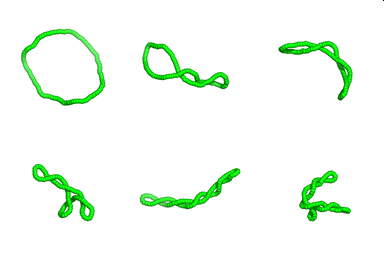
\includegraphics[width=0.768\textwidth,height=0.516\textwidth]{TWsnap.png}
\end{center}
\caption{Sketch of ring polymers with different degree of twisting}
\label{fig:mMemberedTwistedRing}
\end{figure}

\begin{align}
P_{mr}(q) & = I_0\left(\frac{P_{1r}(q)}{m} + \frac{2}{m^2}P_{1r}^2(q)\sum_{j=1}^{m-1}(m-j)\exp\left(-\frac{q^2R^2_{g,1r}}{2}(j-1)\right)\right) \\
P_{1r}(q) & = \sqrt{\frac{2}{u_{1r}^2}} D\left[ \sqrt{\frac{u_{1r}^2}{2}} \right] \\
u_{1r}^2 &= q^2R^2_{g,1r} \\
R^2_{g,1r} &= \sqrt{\frac{b^2N}{12}} \\
D(X) &= \exp\left(X^2\right) \int_0^X \exp(t^2)\, \mathrm{d}t
\end{align}
The above formula is defined for integer values of $m$ larger or equal 1. For non-integer values of $m$ a mixture between $\lfloor m\rfloor$ and $\lfloor m\rfloor+1$ is assumed where $\lfloor m \rfloor$ denotes the greatest integer less than or equal to $m$. (\texttt{\texttt{floor}}-function). We finally get
\begin{align}
P_r{q} &= (1-w)P_{\lfloor m\rfloor r}(q) + w P_{(\lfloor m\rfloor+1) r}(q)
\end{align}
with $w=m-\lfloor m\rfloor$.

\vspace{5mm}

\noindent
\uline{Input Parameters for model \texttt{mMemberedTwistedRing}:}
\begin{description}
\item[\texttt{R\_G,1r}] radius of gyration $R_{G,1r}$ of one of $m$ loop
\item[\texttt{m}]  number of twists $m$
\item[\texttt{I0}] forward scattering $I_0$
\end{description}

\begin{figure}[htb]
\begin{center}
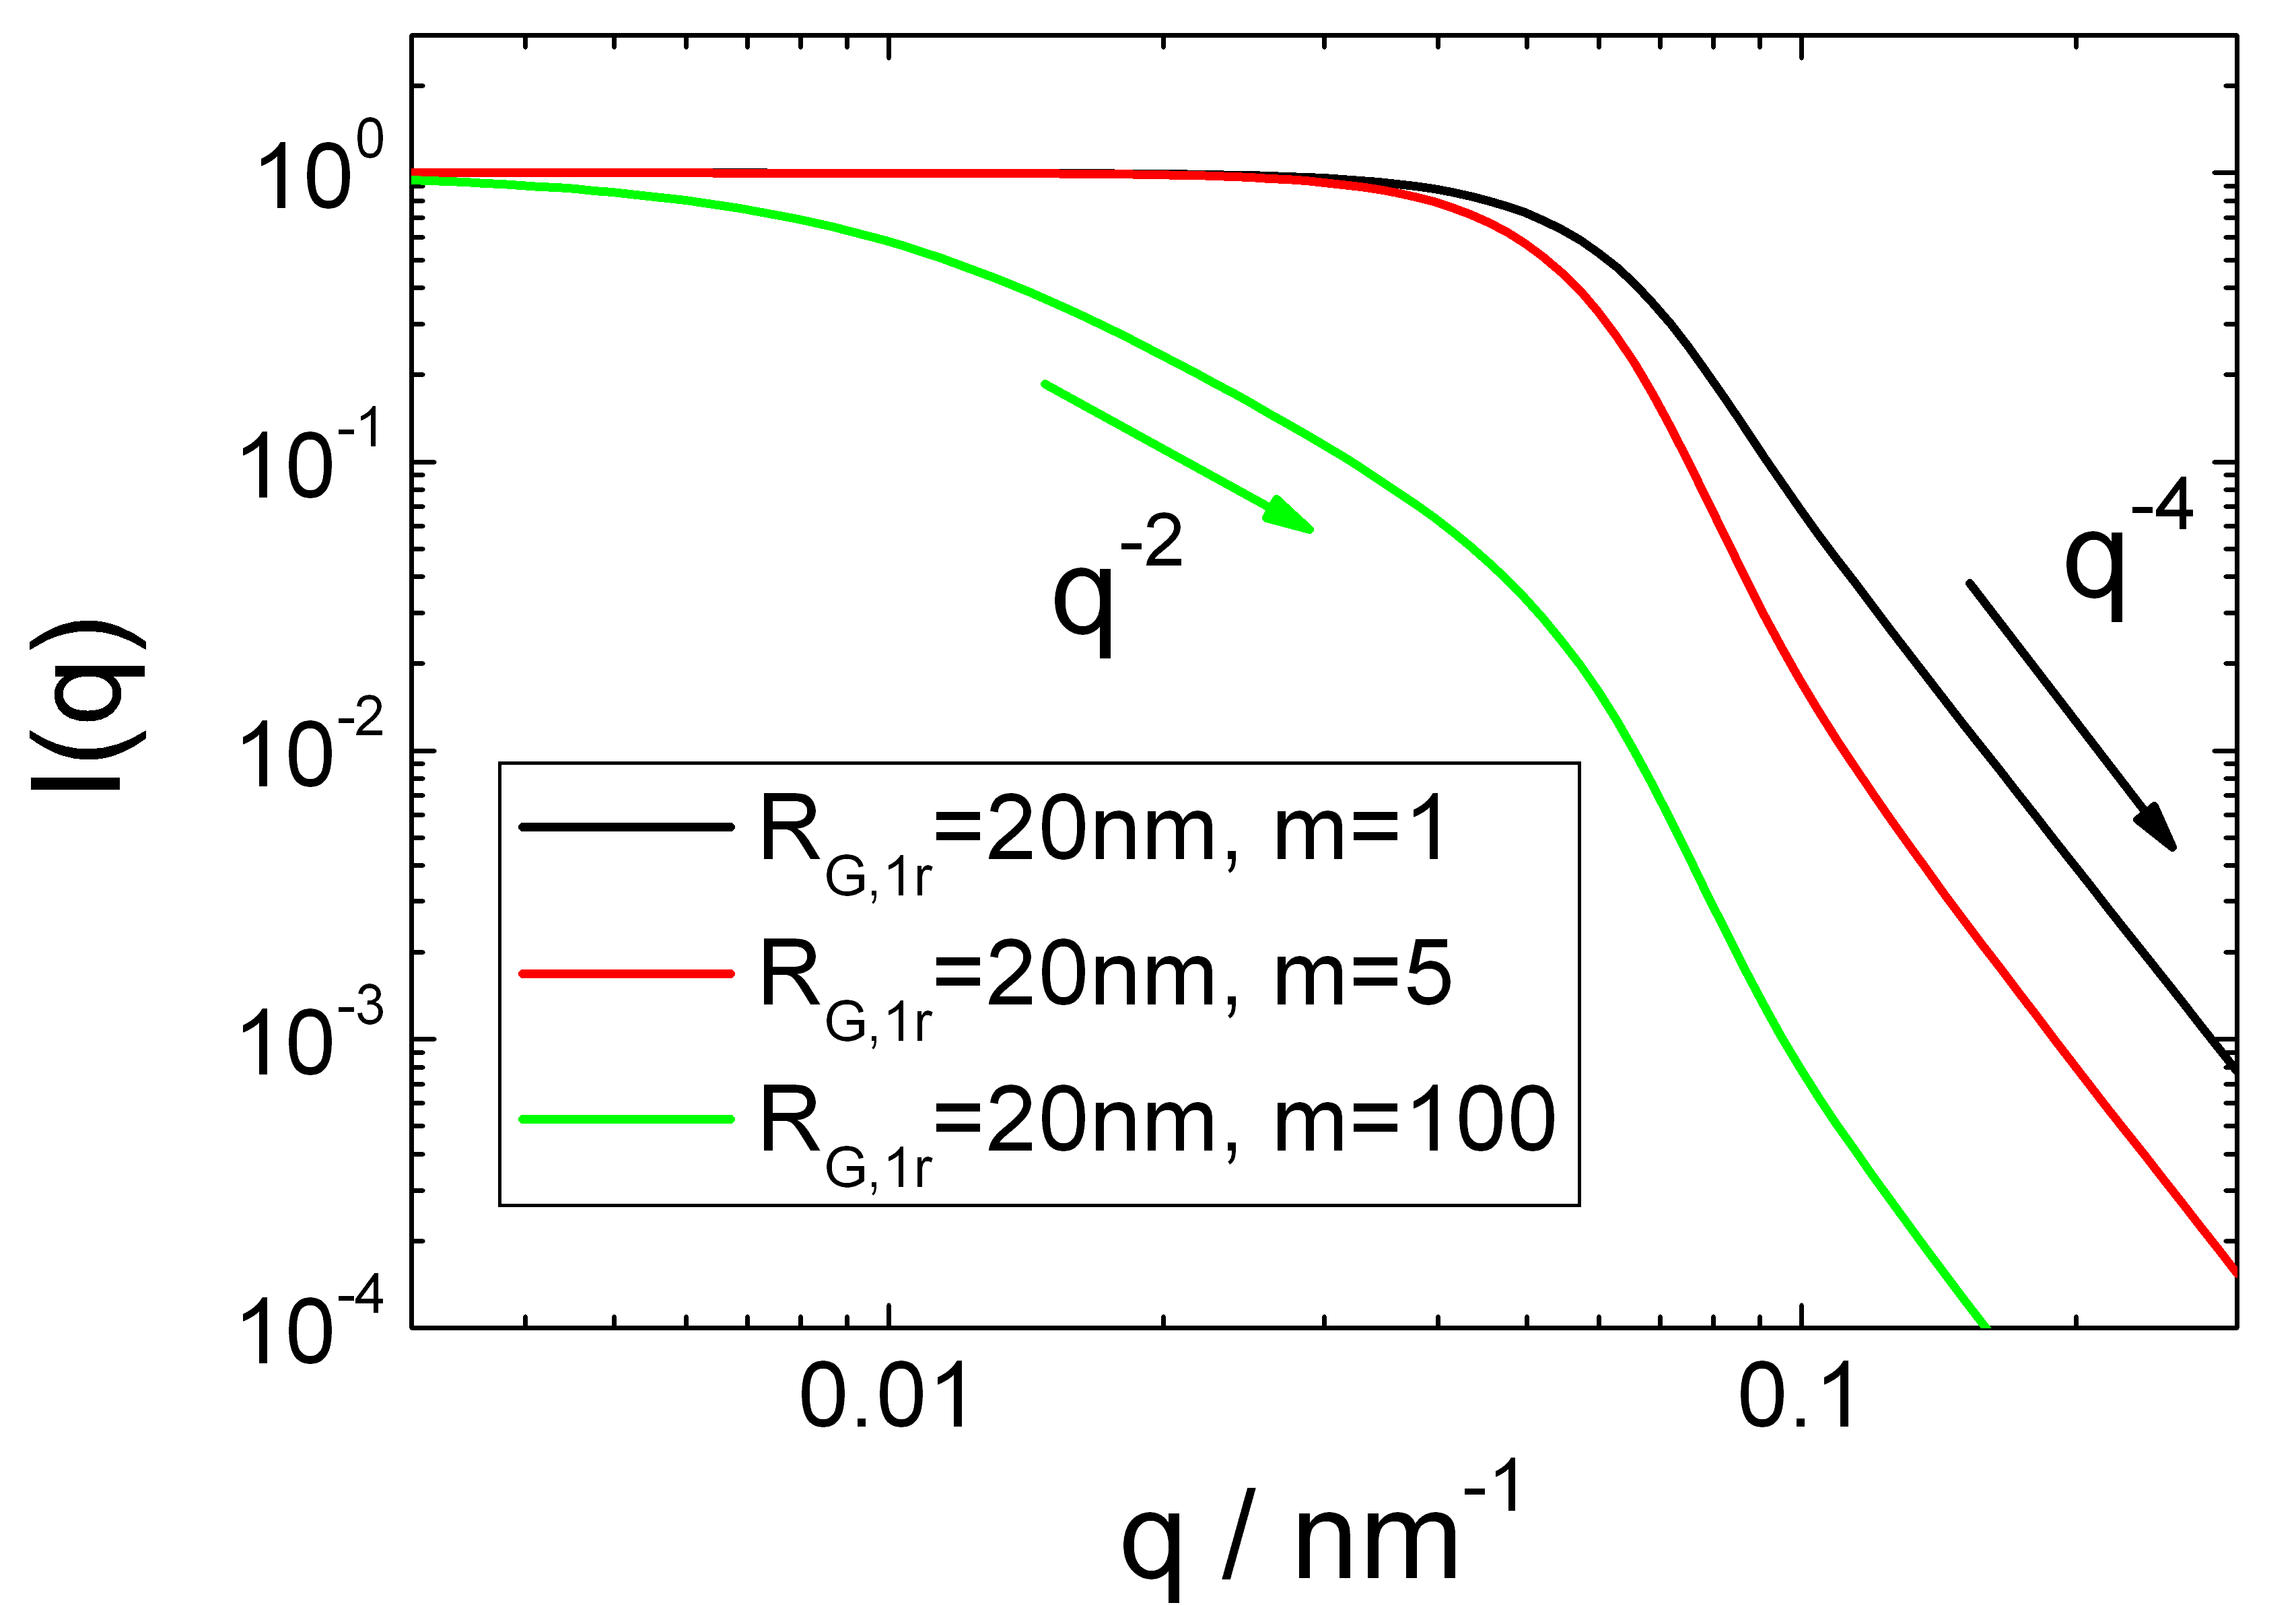
\includegraphics[width=0.768\textwidth]{../images/form_factor/polymer_rings/mMemberedTwistedRing.png}
\end{center}
\caption{Scattering intensity of an $m$-membered twisted ring polymers with different values for $m$.} \label{fig:mMemberedTwistedRingIQ}
\end{figure}

%%%%%%%%%%%%%%%%%%%%%%%%%%%%%%%%%%%%%%%%%%%%%%%%%%%%%%%%%%%%%%%%%%%%%%%%

\clearpage
\subsubsection{Daisy-like Ring}
\label{sect:DaisyLikeRing}
~\\
 \cite{Burchard1996}
\begin{figure}[htb]
\begin{center}
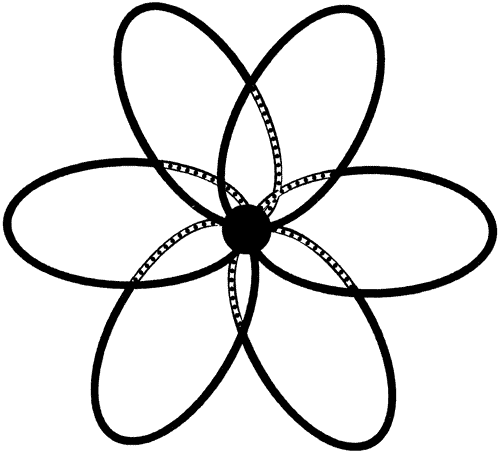
\includegraphics[width=0.5\textwidth,height=0.453\textwidth]{ma9603286f00001.png}
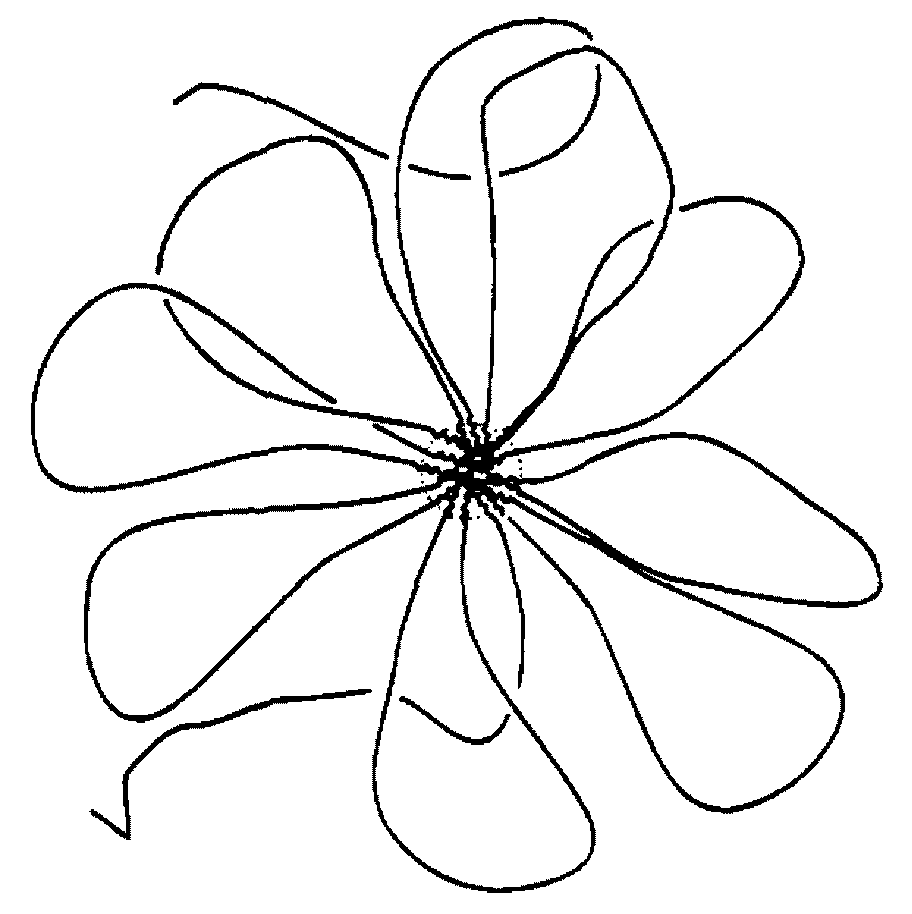
\includegraphics[width=0.45\textwidth,height=0.45\textwidth]{RosetteLikeMicelle.png}
\end{center}
\caption{Sketch of a Daisy-like polymer.}
\label{fig:DaisyLike}
\end{figure}

\begin{align}
P_{mr}(q) & = \frac{I_0}{m}\left(P_{1r}(q) + (m-1)P_{1r}^2(q)\right) \\
P_{1r}(q) & = \sqrt{\frac{2}{u_{1r}^2}} D\left[ \sqrt{\frac{u_{1r}^2}{2}} \right] \\
u_{1r}^2 &= q^2R^2_{g,1r} \\
R^2_{g,1r} &= \sqrt{\frac{b^2N}{12}} \\
D(X) &= \exp(X^2) \int_0^X \exp(t^2)\, \mathrm{d}t
\end{align}

\vspace{5mm}

\noindent
\uline{Input Parameters for model \texttt{DaisyLikeRing}:}
\begin{description}
\item[\texttt{R\_G,1r}] radius of gyration $R_{G,1r}$ of one of $m$ loop
\item[\texttt{m}]  number of loops $m$
\item[\texttt{I0}] forward scattering $I_0$
\end{description}

\begin{figure}[htb]
\begin{center}
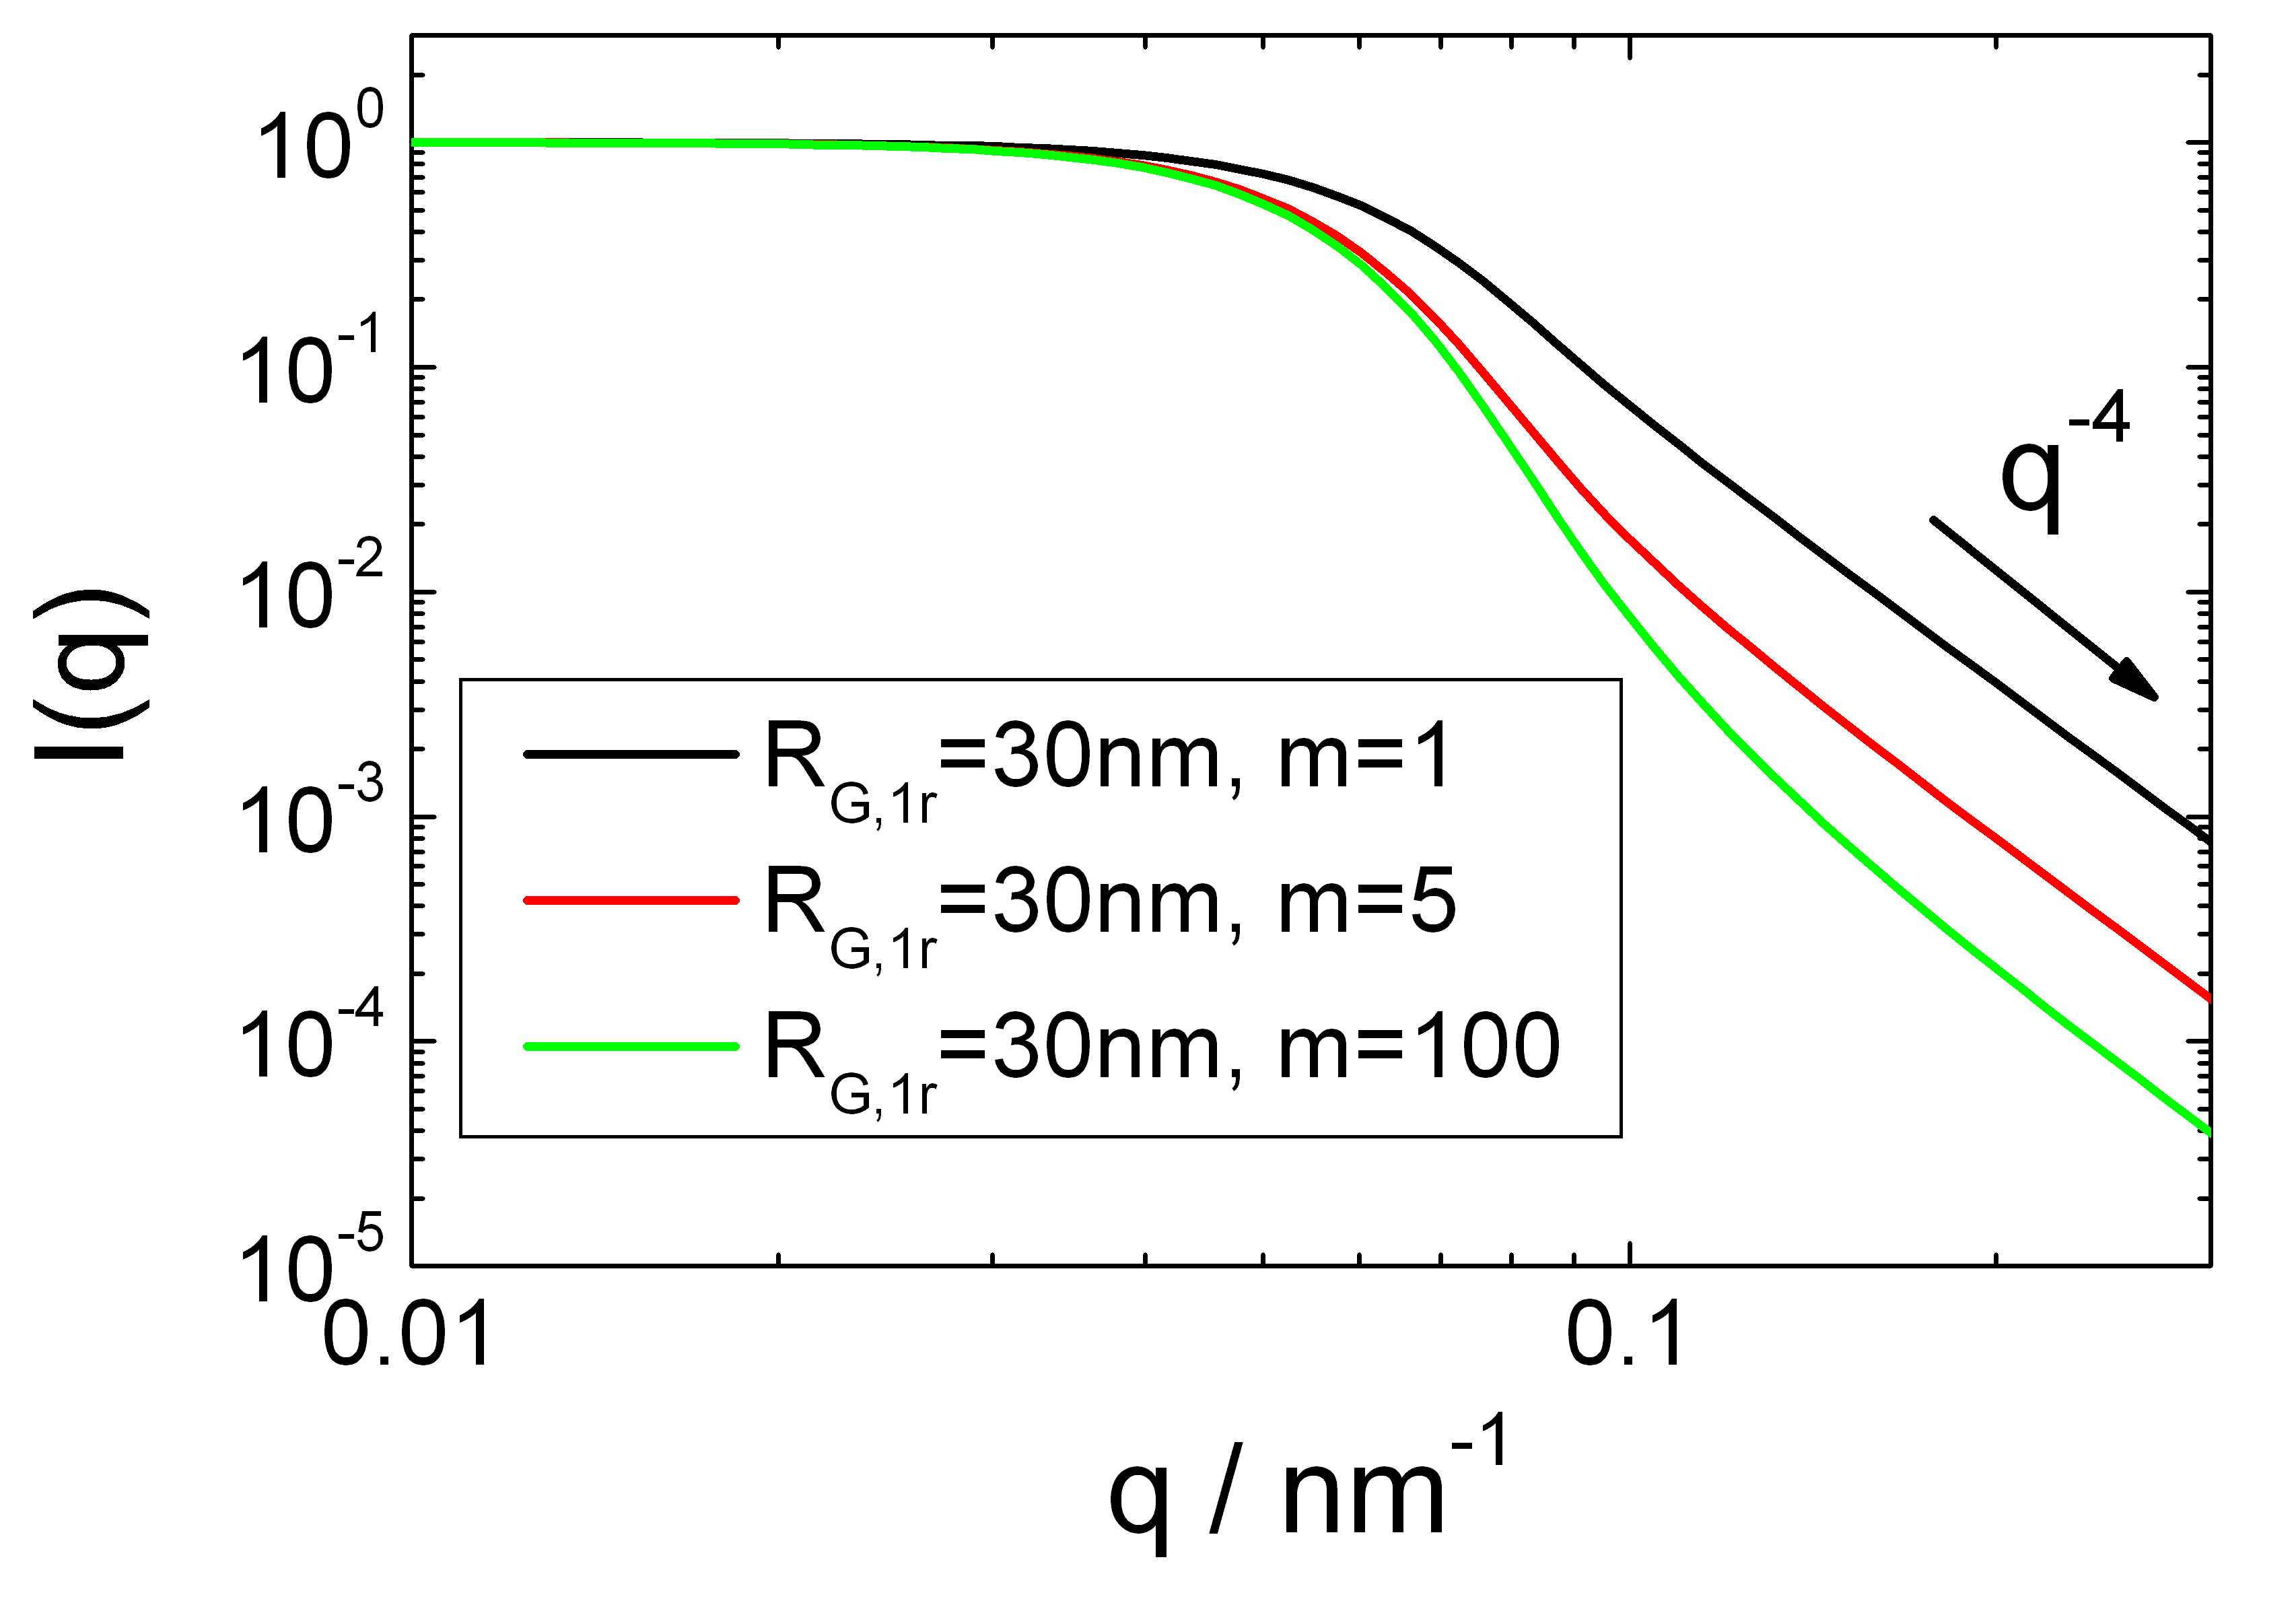
\includegraphics[width=0.768\textwidth]{../images/form_factor/polymer_rings/DaisyRingIQ.png}
\end{center}
\caption{Scattering intensity of a Daisy-like ring polymers with different number of loops.} \label{fig:DaisyRingIQ}
\end{figure}
%%%%%%%%%%%%%%%%%%%%%%%%%%%%%%%%%%%%%%%%%%%%%%%%%%%%%%%%%%%%%%%%%%%%%%%

\clearpage
\subsection{Semi-flexible or worm-like polymers}
\label{sect:semiflexiblePolymers}
~\\

Semi-flexible or worm-like structures have been implemented also as $P'(Q)$ for thin objects with local cylindrical geometry section  \ref{plugin:Pprime4cylindrical}. Here they are implemented for describing polymers with infinitesimal thin cross sections of the stiff Kuhn segments.
\begin{figure}[htb]
\captionsetup[subfigure]{position=b}
\centering
\subcaptionbox{Comparison of semi-flexible polymers without excluded volume effects \label{fig:IQ:WormsComparison1} }{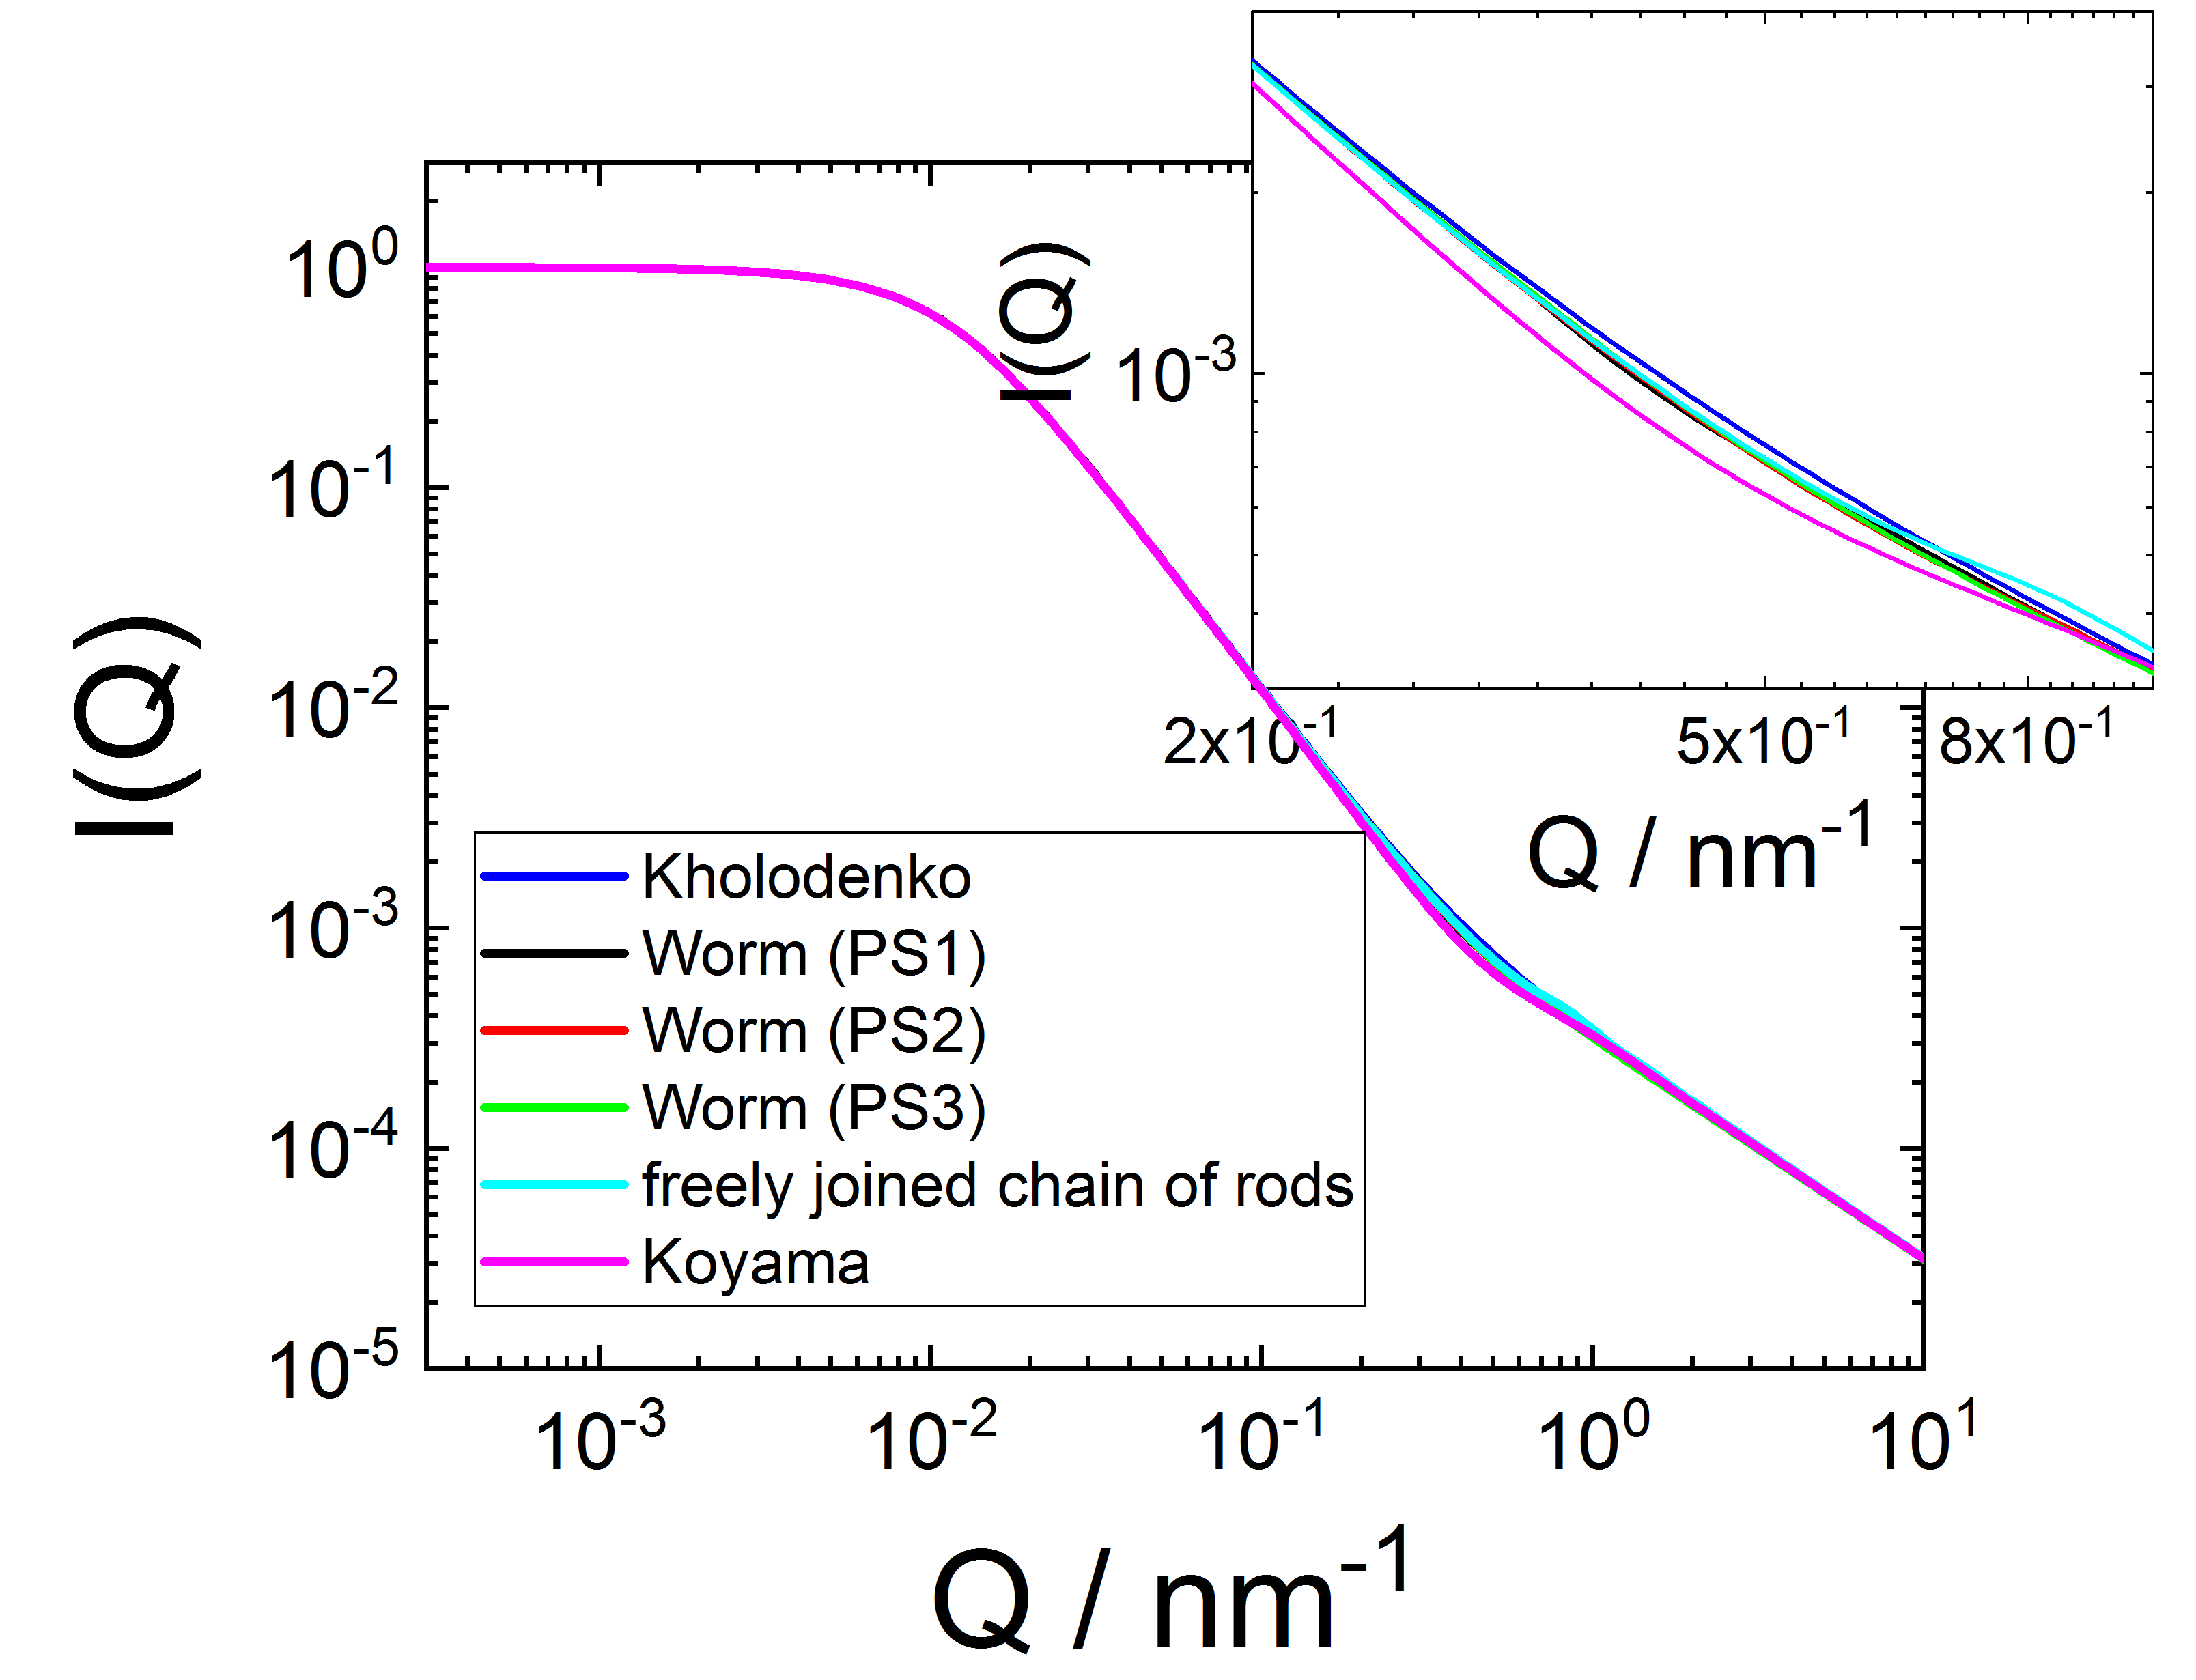
\includegraphics[width=0.48\textwidth]{../images/form_factor/polymer_semiflexible/WormsComparison.png}}
\hfill
\subcaptionbox{Kratky plot of the same data as on the left. \label{fig:IQ:WormsComparison2} }{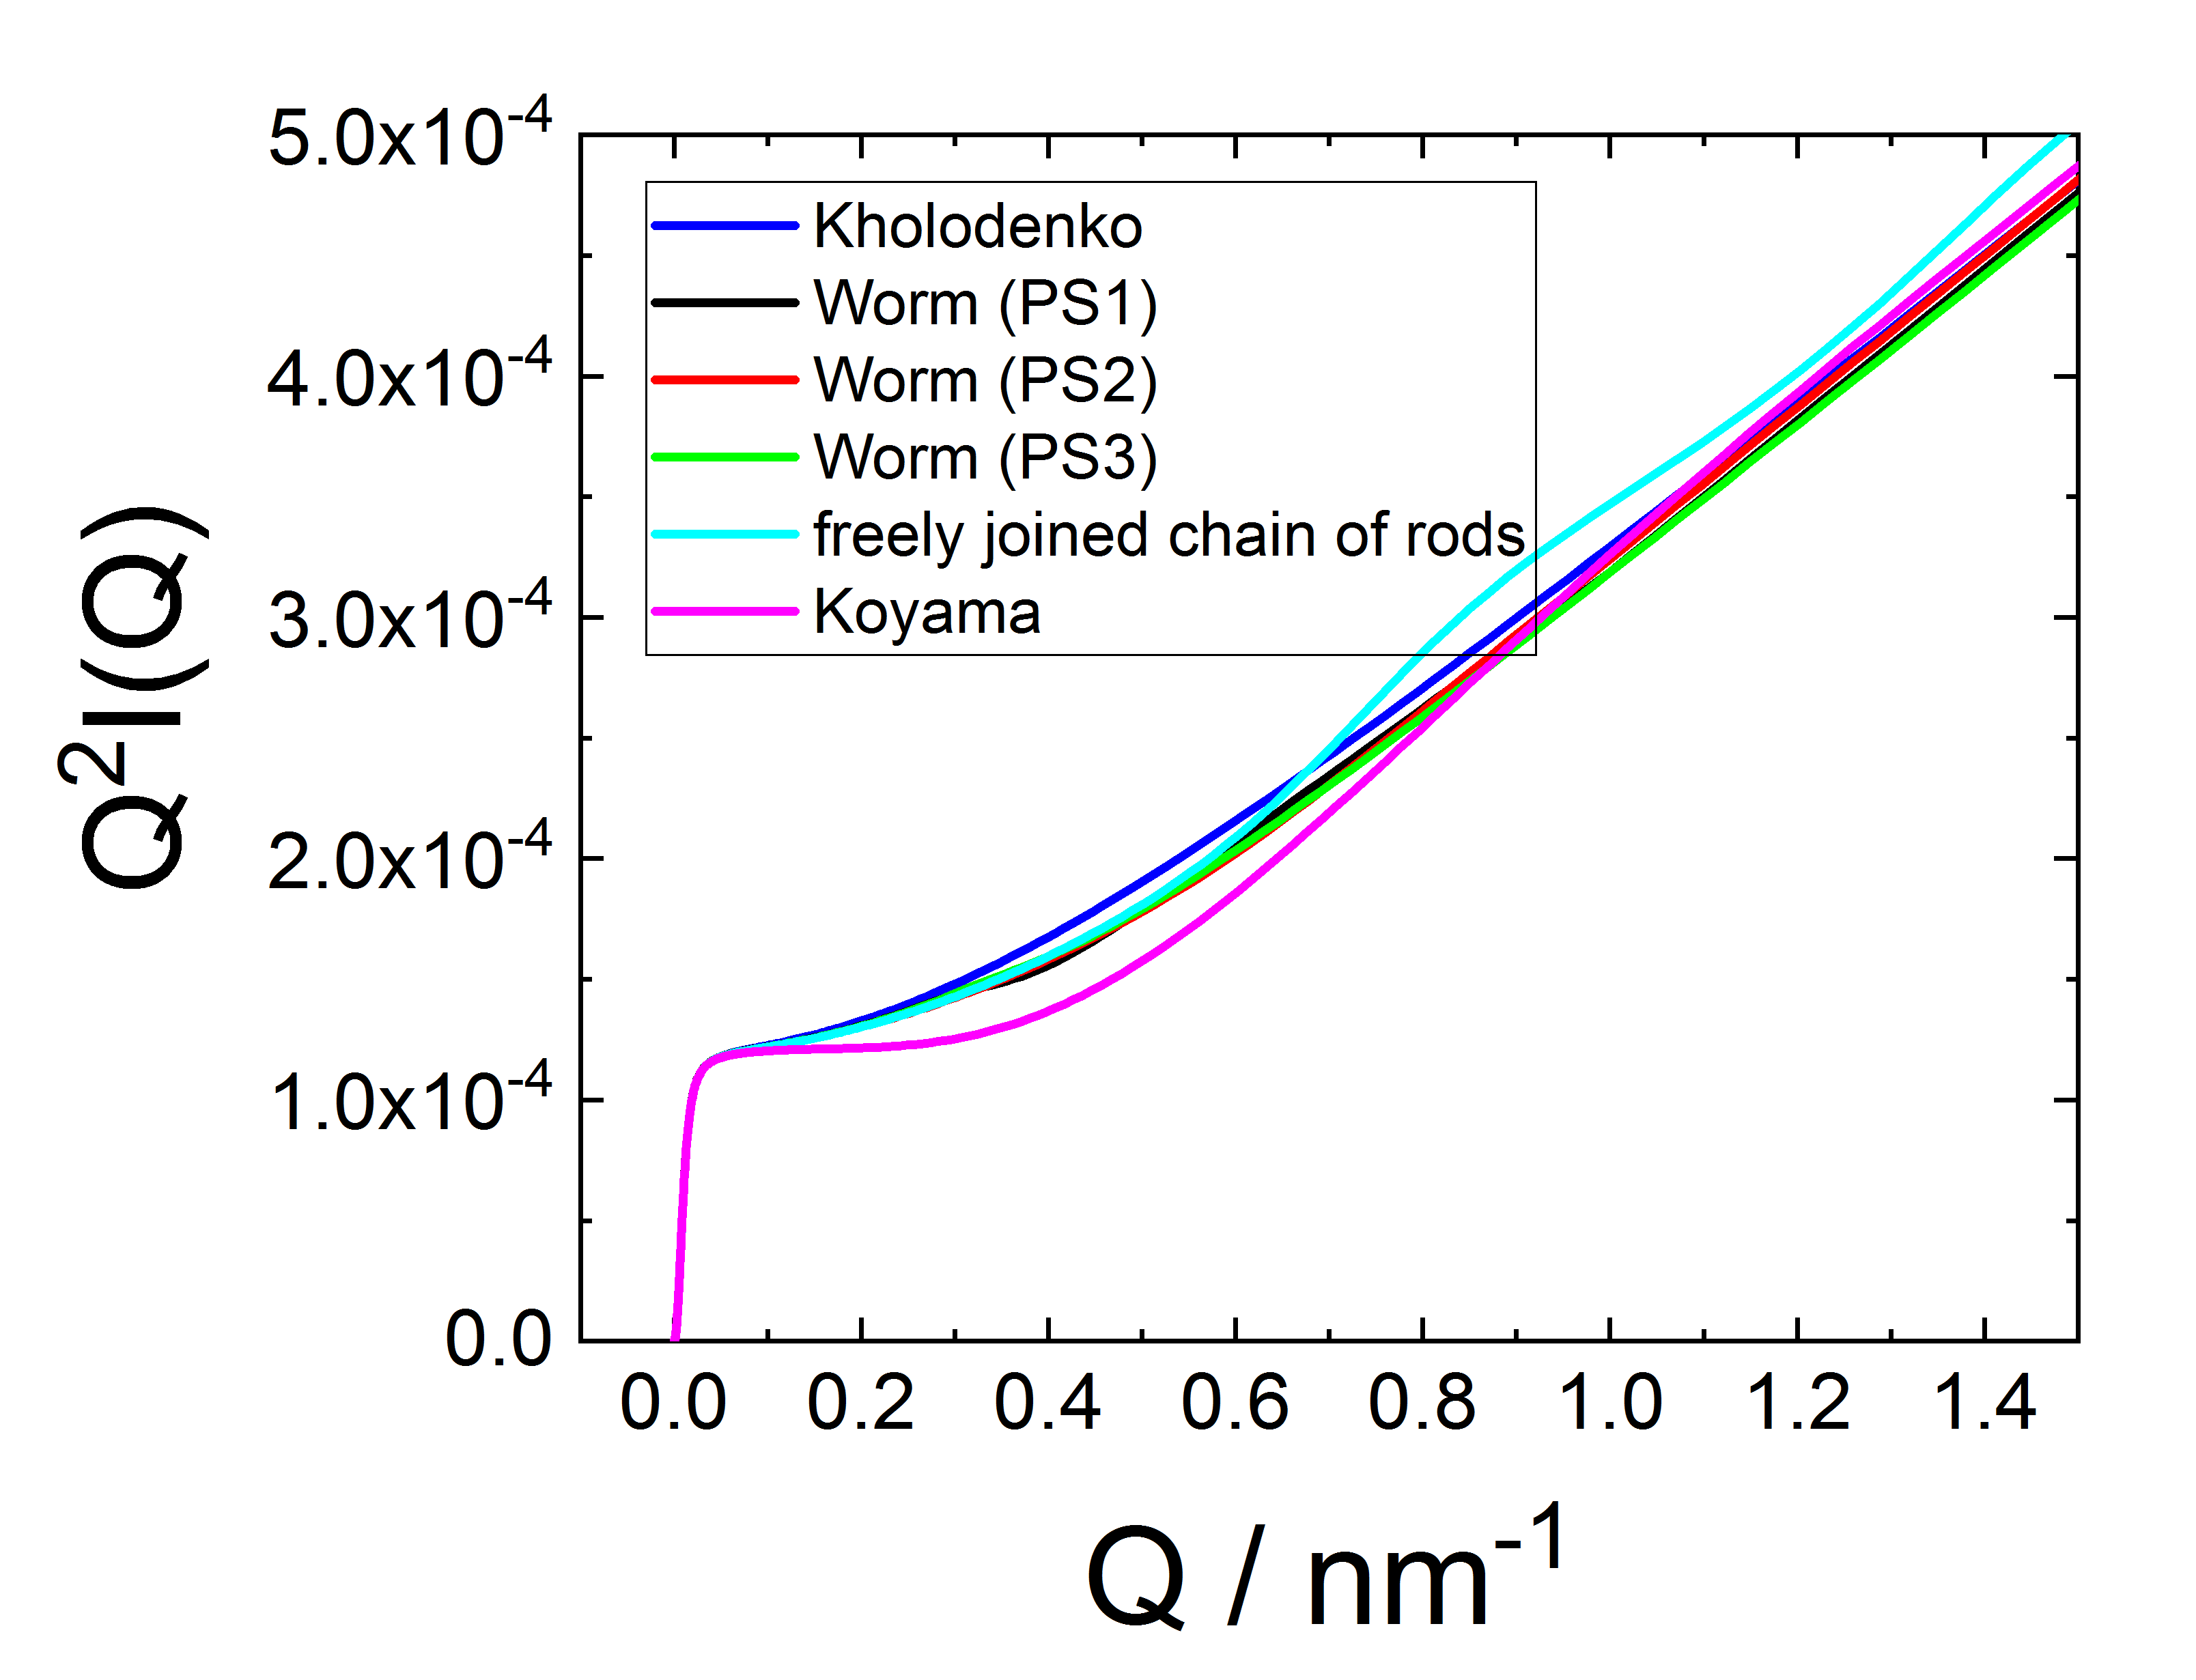
\includegraphics[width=0.48\textwidth]{../images/form_factor/polymer_semiflexible/WormsComparisonKratky.png}}
\caption{Comparison of model for semi-flexible or worm-like polymers}
\label{fig_IQ:WormsComparison}
\end{figure}
~\\

\subsubsection{wormlike polymer (PS1)}
\label{sect:ffWorm(PS1)}
~\\
This first form factor for a semi-flexible polymer without excluded volume effects according to \cite{Pedersen96Macrom} is given in eq.\ \ref{eq:SWC} and with excluded volume effects in eq.\ \ref{eq:exvSWC}. The form factors is normalized to $I(Q=0)=I_0$.

\vspace{5mm}

\hspace{1pt}\\
\uline{Input Parameters for model \texttt{Worms(PS1)} (with and without excluded volume effects):}\\
\begin{description}
\item[\texttt{lb}] Kuhn length $l_B$ of semi-flexible worm-like structure
\item[\texttt{L}] contour length $L$ of semi-flexible worm-like structure
\item[\texttt{exvol}] input flag to select the variant with or without excluded volume effects: $\mathrm{exvol} \geq 1$ with excluded volume effects, $\mathrm{exvol} < 1$ without excluded volume effects
\item[\texttt{I0}] forward scattering $I(Q=0)=I_0$
\end{description}

\vphantom{.}~\\

\subsubsection{wormlike polymer (PS2)}
\label{sect:ffWorm(PS2)}
~\\
This second form factor for a semi-flexible polymer  according to \cite{Pedersen96Macrom} only is available without excluded volume effects and is given in eq.\ \ref{eq:PprimePS2}. The form factors is normalized to $I(Q=0)=I_0$.

\vspace{5mm}

\hspace{1pt}\\
\uline{Input Parameters for model \texttt{Worms(PS2)}:}\\
\begin{description}
\item[\texttt{lb}] Kuhn length $l_B$ of semi-flexible worm-like structure
\item[\texttt{L}] contour length $L$ of semi-flexible worm-like structure
\item[\texttt{dummy}] not used
\item[\texttt{I0}] forward scattering $I(Q=0)=I_0$
\end{description}

\vphantom{.}~\\

\subsubsection{wormlike polymer (PS3)}
\label{sect:ffWorm(PS3)}
~\\
This third form factor for a semi-flexible polymer without excluded volume effects according to \cite{Pedersen96Macrom} is given in eq.\ \ref{eq:PprimePS3} for both without and with excluded volume effects. The form factors is normalized to $I(Q=0)=I_0$.

\vspace{5mm}

\hspace{1pt}\\
\uline{Input Parameters for model \texttt{Worms(PS3)} (with and without excluded volume effects):}\\
\begin{description}
\item[\texttt{lb}] Kuhn length $l_B$ of semi-flexible worm-like structure
\item[\texttt{L}] contour length $L$ of semi-flexible worm-like structure
\item[\texttt{exvol}] input flag to select the variant with or without excluded volume effects: $\mathrm{exvol} \geq 1$ with excluded volume effects, $\mathrm{exvol} < 1$ without excluded volume effects
\item[\texttt{I0}] forward scattering $I(Q=0)=I_0$
\end{description}

\vphantom{.}~\\

\subsubsection{Kholodenko worm}
\label{sect:ffKholodenkoWorm}
~\\
Kholodenko \cite{kholodenko93} has given a simple expression for semi-flexible polymers without excluded volume effects. The form factor has been given in section \ref{plugin:Pprime4kohlodenko} by eq.\ \ref{eq:KholodenkoPprime}. The form factors here is normalized to $I(Q=0)=I_0$.

\vspace{5mm}

\hspace{1pt}\\
\uline{Input Parameters for model \texttt{Kholodenko worm}:}\\
\begin{description}
\item[\texttt{lb}] Kuhn length $l_B$ of semi-flexible worm-like structure
\item[\texttt{L}] contour length $L$ of semi-flexible worm-like structure
\item[\texttt{dummy}] not used
\item[\texttt{I0}] forward scattering $I(Q=0)=I_0$
\end{description}

\vphantom{.}~\\

\subsubsection{Koyama worm}
\label{sect:ffKoyamaWorm}
~\\
This form factors of semi-flexible polymers from Koyama \cite{Koyama1973,Koyama1974} given in eq.\ \ref{eq:PprimeKoyama} but normalized here to $I(Q=0)=I_0$.

\vspace{5mm}

\hspace{1pt}\\
\uline{Input Parameters for model \texttt{Koyama worm}:}\\
\begin{description}
\item[\texttt{lb}] Kuhn length $l_B$ of semi-flexible worm-like structure
\item[\texttt{L}] contour length $L$ of semi-flexible worm-like structure
\item[\texttt{dummy}] not used
\item[\texttt{I0}] forward scattering $I(Q=0)=I_0$
\end{description}

\vphantom{.}~\\

\subsubsection{Freely joined chain of rigid rods}
\label{sect:ffWormFreelyJoinedChainOfRods}
~\\
The form factors of freely joined chain of rigid rods by Hermans and Hermans \cite{Hermans1958} is given in eq.\ \ref{eq:PprimeFreelyJoinedRods} but normalized here to $I(Q=0)=I_0$.

\vspace{5mm}

\hspace{1pt}\\
\uline{Input Parameters for model \texttt{freely joined chain of rods}:}\\
\begin{description}
\item[\texttt{lb}] Kuhn length $l_B$ of semi-flexible worm-like structure
\item[\texttt{L}] contour length $L$ of semi-flexible worm-like structure
\item[\texttt{dummy}] not used
\item[\texttt{I0}] forward scattering $I(Q=0)=I_0$
\end{description}

\clearpage
\subsection{branched polymer}
\label{sect:branched_polymers}
~\\
Polymers can be synthesized in a large variety of architectures, like architectures of linear polymers, rings, branched polymers, dendrimers, combs, ladders, cross-linked polymers, etc. A few possible architectures are sketched in fig.\ \ref{fig:polymer_architectures}.

\begin{figure}[htb]
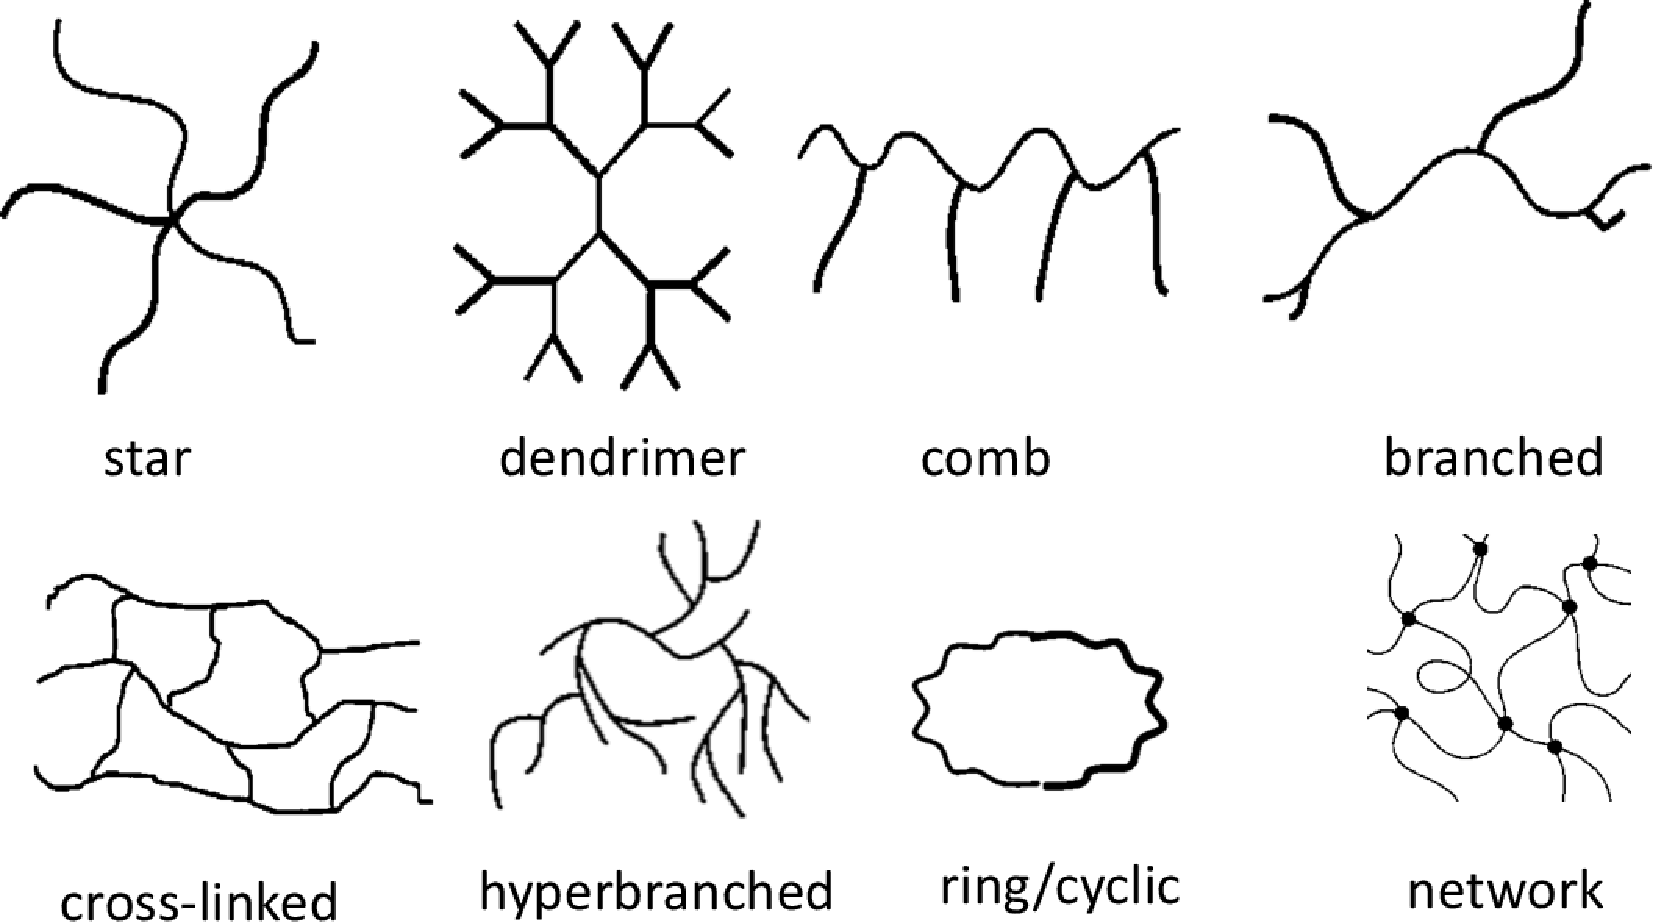
\includegraphics[width=0.8\textwidth]{../images/form_factor/polymer_branched/polymer_architectures.pdf}
\caption{Some categories of polymer architectures}
\label{fig:polymer_architectures}
\end{figure}


~\\
\subsubsection{random $f$-functional polycondensates}
\label{sect:ff_functional_homopolycondensates}
~\\
\cite{Kajiwara1970,Burchard2015,Burchard2015a,Burchard1977}
\begin{align}\label{eq:f-functionalHomoPolym}
  I_{f-\mathrm{pc}} &= \frac{I_0}{1+R_g^2q^2/3} \\
  R_g^2 &= \frac{1}{2}\sigma^2 \left(\frac{\alpha(f-1)}{1-\alpha(f-1)}+\frac{\alpha}{1+\alpha}\right)
\end{align}
where $f$ is the functionality, $\alpha$ the fraction of functionalities which have reacted and $\sigma^2$ may be defined as the mean-square distance between two units directly connected by a link.

~\\
\subsubsection{hyperbranched polymer: fractal approach}
\label{sect:ffhyperbranched_fractal}
~\\

\cite{Burchard2004}


~\\
\subsubsection{Hyper-branched $AB_2$ polymers perturbed by excluded
volume interaction}
\label{sect:ffhyperbranched_exvol}
~\\

\cite{Burchard2015,Burchard2015a}

~\\
\subsubsection{comb}
\label{sect:com}
~\\
Casassa and Berry have developed a model polymers with a comb-like architecture \cite{Casassa1966}. They assume sufficiently dilute solution at the Flory temperature, where the molecular configuration is described by random flight statistics. They describe in their paper three version, a regular, a random and a heterogenous comb architecture.

The form factor of a regular comb reads as \cite{Casassa1966,von_Ferber_2013}
\begin{align}\label{eq:comb_regular}
  I_\mathrm{comb,reg}(q) &=  \frac{2}{x^2}\left(A_\mathrm{reg}+B_\mathrm{reg}+C_\mathrm{reg}\right)\\
  A_\mathrm{reg} &= x-1+e^{-x\lambda}\\
  B_\mathrm{reg} &= \left(1-e^{-x(1-\lambda)/\zeta} \right)\left(\zeta+2\frac{1-e^{-x\lambda \zeta/(\zeta+1)}}{1-e^{x\lambda/(\zeta+1)}}\right)\\
  C_\mathrm{reg} &=  \left(1-e^{-x(1-\lambda)/\zeta} \right)^2 \\ &\phantom{=} \qquad \left(\frac{(\zeta-1)\left(e^{x\lambda/(\zeta+1)}-1\right)-\left(1-e^{-x\lambda(\zeta-1)/(\zeta+1)}\right)}{\left(1-e^{x\lambda/(\zeta+1)}\right)^2}\right) \nonumber
  \end{align}
with
\begin{align}
  x & = q^2a^2 \\
  a^2 = N l_b^2 /6 \\
  N &= N_0+\zeta n_\zeta \\
  \lambda &= N_0/N
\end{align}
where $l_b$ is the length of a polymer chain element, $\zeta$ the number of side branches equally spaced along the back-bone, $N$ the total number of chain (Kuhn) elements, $N_0$ the chain elements in the back-bone, $n_\zeta$ the number of chain elements in the side branch. $a$ would be the radius of gyration of a linear polymer withe the same number of chain elements than the comb shaped polymer.

The form factor of a random comb reads as \cite{Casassa1966}
\begin{align}\label{eq:comb_random}
  I_\mathrm{comb,rnd}(q) &=  \frac{2}{x^2}\left(A_\mathrm{rnd}+B_\mathrm{rnd}+C_\mathrm{rnd}\right)\\
  A_\mathrm{rnd} &= x + \left(e^{-x\lambda}-1\right)\\
  B_\mathrm{rnd} &= \left(1-e^{-x(1-\lambda)/\zeta}\right)\zeta\left[1+\frac{2}{x\lambda}\left(e^{-x\lambda}-1\right)\right]\\
  C_\mathrm{rnd} &= \left(1-e^{-x(1-\lambda)/\zeta}\right)^2 \left[\frac{x\lambda+\left(e^{-x\lambda}-1\right)}{x^2\lambda^2/(\zeta(\zeta-1))}\right]
\end{align}

The third case discussed in \cite{Casassa1966} includes a binomial distributed random $\zeta$-branched comb, which they name heterogenous. The averaged random form factor (heterogeneous comb) reads as
\begin{align}\label{eq:comb_h}
  I_\mathrm{comb,h}(q) &=  \frac{2}{\bar{x}^2}\frac{1}{1+(1-\bar{\lambda})^2/\bar{\zeta}}\left(A_\mathrm{h}+B_\mathrm{h}+C_\mathrm{h}\right)\\
  A_\mathrm{h} &= \bar{x} + \left(e^{-\bar{x}\bar{\lambda}}-1\right)\\
  B_\mathrm{h} &= \left(1-e^{-\bar{x}(1-\bar{\lambda})/\bar{\zeta}}\right)\bar{\zeta}\left[1+\frac{2}{\bar{x}\bar{\lambda}}\left(e^{-\bar{x}\bar{\lambda}}-1\right)\right]\\
  C_\mathrm{h} &= \left(1-e^{-\bar{x}(1-\bar{\lambda})/\bar{\zeta}}\right)^2 \left[\frac{\bar{x}\bar{\lambda}+\left(e^{-\bar{x}\bar{\lambda}}-1\right)}{\bar{x}^2\bar{\lambda}^2/\bar{\zeta}^2}\right]
\end{align}
where $\bar{x}$, $\bar{\lambda}$, and $\bar{\lambda}$ are averaged accordingly (details see \cite{Casassa1966}).
In fig.\ \ref{fig:comb} The scattering intensity of am comb with 10 branches is shown. The differences between the models are hardly visible in the loglog presentation, however, in the Kratky plot they become visible.
\begin{figure}[htb]
\begin{center}
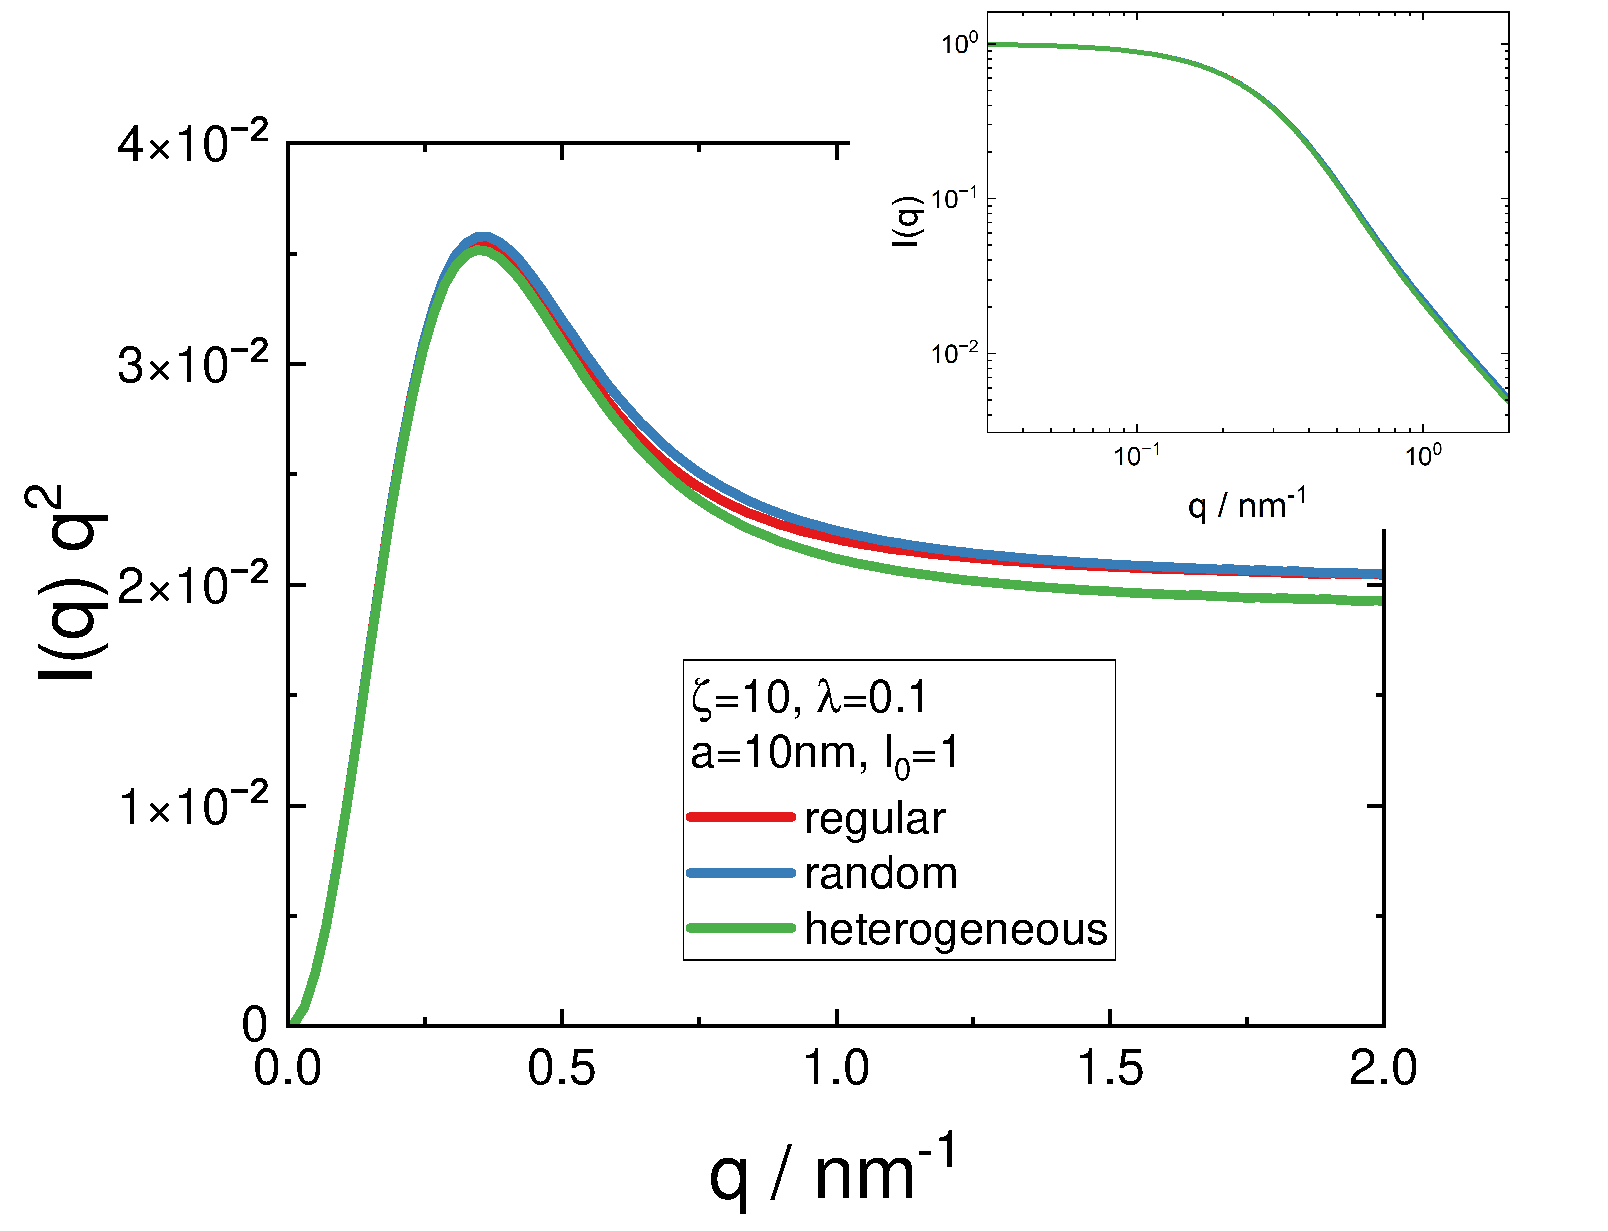
\includegraphics[width=0.8\textwidth]{../images/form_factor/polymer_branched/comb.pdf}
\end{center}
\caption{Scattering of a comb in a Kratky and Loglog plot.}
\label{fig:comb}
\end{figure}

\noindent \uline{Input Parameters for models \texttt{comb (regular)}, \texttt{comb (random)}, and \texttt{comb} \texttt{(heterogeneous)}:}\\
\begin{description}
\item[\texttt{a}] radius of gyration of a linear chain with the same number of polymer units $a$ as the comb
\item[\texttt{zeta}] functionality or number of branches $\zeta$
\item[\texttt{lambda}] density of side chains $\lambda$
\item[\texttt{I0}] forward scattering $I_0$
\end{description}

\noindent\uline{Note:}
\begin{itemize}
\item $0\leq \lambda \leq 1$
\item $\zeta > 1$
\item $a>0$
\end{itemize}

~\\
\subsubsection{bottle-brush polymer}
\label{sect:com_regular}
~\\
\begin{figure}[htb]
\begin{center}
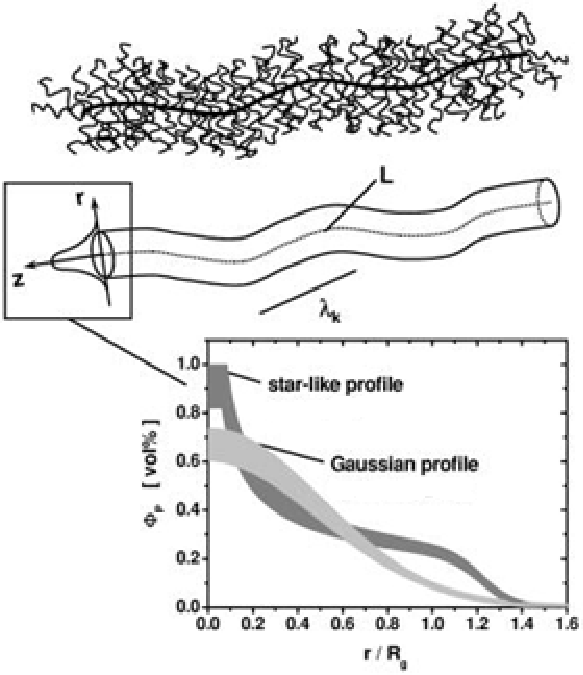
\includegraphics[width=0.5\textwidth]{../images/form_factor/polymer_branched/bottle_brush_polymer.pdf}
\end{center}
\caption{sketch of a bottle brush polymer \cite{Rathgeber2005}.}
\label{fig:bottlebrush}
\end{figure}

For a bottle-brush polymer analytical expressions for the scattering length density profile of the brush cross-section have been suggested by \cite{Rathgeber2005}, which is an empirical star-like profile, and by \cite{Hsu2007,Hsu2008} based on simulations.
The corresponding profiles read as
\begin{align}
  \rho_\mathrm{emp}(r) &= 
    \begin{cases}
      \eta , & \mbox{if } r\leq R_c \\
      \eta \alpha r^{-k}\left\{1+\exp\left(\frac{r-R_s}{\sigma_s}\right)\right\}^{-1}, & \mbox{otherwise}.
    \end{cases}
  \label{eq:xsBrushes1}\\
  \rho_\mathrm{sim}(r) &= \frac{\sigma \eta}{1+\left(r/R_1\right)^{x_1}} \exp\left[-\left(r/R_2\right)^{x_2}\right]\label{eq:xsBrushes2}
\end{align}
with $\eta$ being the scattering contrast, $\alpha=R_c^k\left\{1+\exp\left(\frac{R_c-R_s}{\sigma_s}\right)\right\}$ a scaling constant so that $\rho(R_c)$ is continuous, $R_c$ the inner radius, up to which this profile is constant, $k$ describes the power law decay to some outer radius $R_s$ with $\sigma_s$ to have a smooth transition to zero (Fermi function). In the second model $\sigma$ describes the grafting density, $R_1$ and $R_2$ are the length scales for the algebraic decays ($R_1 \ll R_2$), and $x_1$ and $x_2$ are the corresponding exponents. It is expected to have $x_1\simeq (3\nu-1)/(2\nu)$, where $\nu$ is the Flory parameter.

For this two profiles the cross-section term $P_\mathrm{cs}(q)$ for thin rod-like structures as discussed in \ref{sec:very_anisotropic_particles}  using eq.\ \ref{Pcs:cylindrical} reads as
\setstackgap{L}{0.3\baselineskip}
\begin{align}
P_\textrm{cs}^{\mathstack{\text{\tiny emp}}{\text{\tiny sim}}} (q) = \left[2\pi\int_0^\infty
\rho_{\mathstack{\text{\tiny emp}}{\text{\tiny sim}}}(r) \textrm{J}_0(qr)r \,
\textrm{d}r\right]^2 \label{Pcs:bottlebrush}
\end{align}

\noindent \uline{Input Parameters for models  \texttt{BottleBrush (emp.)} and \texttt{BottleBrush profile (emp.)}:}\\
\begin{description}
\item[\texttt{eta}] contrast
\item[\texttt{Rc}] core radius $R_c$
\item[\texttt{k}] power law decay $k>0$
\item[\texttt{Rs}] outer radius $R_s > R_c$
\item[\texttt{sigma\_s}] transition width $\sigma_s$
\end{description}

\noindent\uline{Note:}
\begin{itemize}
\item $R_s > R_c $
\item $k > 0$
\item $\sigma_s>0$
\end{itemize}

\noindent \uline{Input Parameters for models \texttt{BottleBrush (sim)} and \texttt{ BottleBrush profile (sim)}:}\\
\begin{description}
\item[\texttt{sigma\_eta}] grafting density times scattering contrast $\sigma \eta$
\item[\texttt{R\_1}] first length scales for the algebraic decays $R_1$
\item[\texttt{x\_1}] first power law decay $x_1>0$
\item[\texttt{R\_2}] second length scales for the algebraic decays $0<R_1 \ll R_2$
\item[\texttt{x\_2}] second power law decay $x_2>0$
\end{description}

\noindent\uline{Note:}
\begin{itemize}
\item $0< R_1 \ll R_2 $
\item $x_1 > 0$
\item $x_2 > 0$
\end{itemize}

~\\
\subsubsection{soft sphere model}
\label{sect:soft sphere}
~\\
\cite{Savin2004,Burchard,Burchard1982}
